%\documentclass[letterpaper]{sig-alternate}
\documentclass{article}
\usepackage[left=1.0in,right=1.0in,nohead,nofoot]{geometry}
\usepackage{multirow} 
\usepackage{rotating}
\usepackage{listings}
\usepackage{color}
\usepackage{capt-of}
\usepackage{caption}
\usepackage{float}

\begin{document}

%\conferenceinfo{}
%\CopyrightYear{}
%\crdata{}


\title{Software for Embedded Systems\\Hovercraft Project\\Final Report}


\author{Darren Minifie, Marco Yuen, Kat Gunion and Anthony Estey}

\date{April 23, 2009}
\maketitle
\begin{abstract}
Hovercraft report abstract here.
\end{abstract}

\tableofcontents
\listoffigures
\listoftables
\newpage

%A category including the fourth, optional field follows...
%\category{D.2.8}{Software Engineering}{Metrics}[complexity measures, performance measures]

%\terms{}



\section{Introduction}
Writing software for embedded systems poses many challenges that don't exist on larger systems such as desktop computers, severs and even mobile devices.  Severely reduced cpu and memory resources, as well as minimal hardware interface abstractions, requires software to be extremely efficient and correct.  The overall objective of this project is to apply concepts in embedded systems design, as well as first principles of electronics, to construct a completely autonomous hovercraft that can navigate corners and avoid other obstacles.  A seemingly simple task such as this quickly becomes complex with the addition of hardware interface, self-monitoring and autonomous intelligence software.  

The complete project is segmented into three cumulative milestones.  Milestone 1 deals with the interfacing of the various electronic components to an Atmel AT90 microcontroller.  Milestone 2 consists of the design and construction of the hovercraft, the addition of the electronic components to the vehicle, and an analysis of various physical parameters of the hovercraft system.  Finally, milestone 3 realizes the full objective of the project: to supply the hovercraft with intelligence such that it may navigate a given course without coming in contact with any obstacles along the way.  

The graduate level criteria adds yet another objective: the communication and coordination between two hovercrafts.  Accordingly, the design, construction and testing of a second hovercraft is required, as well is supplemental communications software to support inter-vehicle synchronization.

This document describes, in detail, each of the three milestones in terms of their background theory, implementation methodologies, evaluation strategies and formalized results.  

\clearpage
\section{Electronic Components and Their Interface}
This section describes the various electronic components used in the project, as well as their interface to one another.  This section focuses on the hardware / electrical aspect of the components; one should refer to Section \ref{embeddedSoftwareAutomation} for details regarding the software implementation.  

\subsection{Hardware Components}
The following components were attached to an Atmel AT90 microcontroller either directly, or indirectly through a breadboard.  

\subsubsection{Atmel Microcontroller}
The Hovercraft project is centered around the AT90USB1287 processor from Atmel, mounted on a AT90USBKey which is shown in Figure \ref{fig:at90usbkey}.

\begin{minipage}{6.5in}
  \centering
    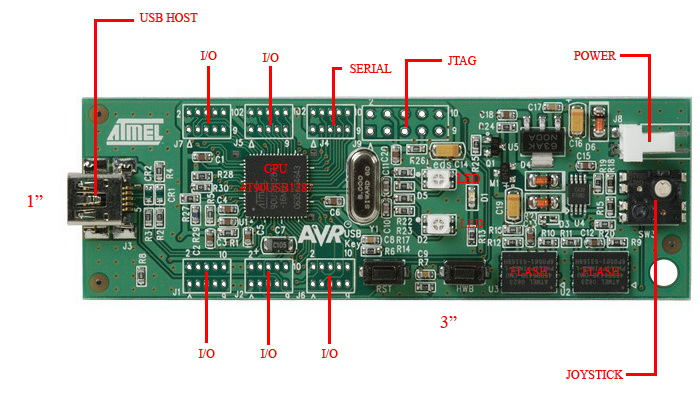
\includegraphics[width=110mm]{imageSources/at90usbkey.png}
 
  \captionof{figure}{Atmel AT90USBkey} 
  \label{fig:at90usbkey}
\end{minipage}

Some of the most notable features of this board include:
\begin{itemize}
\item USB Interface
\item 4+1-ways joystick
\item 2 Bi-Color LEDs
\item temperature sensor
\item serial dataflash memories
\item On-board RESET button 
\item On-board HWB button to force bootloader section execution at reset.
\item System clock: 8 MHz crystal
\end{itemize}

\subsubsection{Radio}
The radio used for hovercraft-basestation and hovercraft-hovercraft communication is the TRW-24G.  The datasheet for this component can be found here.  The radio operates at a frequency of 2.4 to 2.527 GHz and has a working voltage of 3 Volts (ranging from 1.8 to 3.6 Volts).  The radio can transit anywhere from 250 Kbps to 1000 Kbps (1Mbps).  Communication is segmented into 128 distinct channels which each occupy a 1 MHs chunk of spectrum. 

\begin{minipage}{6.5in}
  \begin{center}
    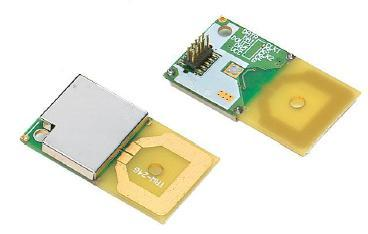
\includegraphics[width=110mm]{imageSources/radio.png}
  \end{center}
  \captionof{figure}{TRM-24G RF 2-way Radio} 
  \label{radioFig}
\end{minipage}

\subsubsection{Motors}
Several types of motors, as well as other supporting circuitry, are required to propel and maneuver the hovercraft.  

The DC Motor

The H-Bridge used is the L293D chip. This chip has the ability to run two H-bridges. 

  \begin{minipage}{6.5in}
        \centering
    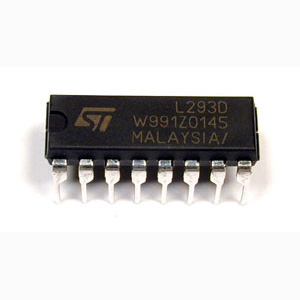
\includegraphics[width=110mm]{imageSources/hBridge.png}
  \captionof{figure}{L2930 H-Bridge} 
  \label{hBridge}
\end{minipage}



The L293D chip contains four input/output channels that can be used as two bridges. Each bridge (i.e. two channels) contains an enable connection required to operate the it. If the enable connection is given HIGH input, channel output is the same as channel input. If the enable is not connected or given LOW input, the channel output will be high impedance always. The L293D chip requires two connections at all times: a supply voltage (+5V) and ground (+0V). The chip also provides a second logic supply voltage if lower voltage operation is required.

The 74HC04 hex inverter chip is very simple. If the chip receives a HIGH signal, it will return a LOW signal, and visa versa. This hex inverter provides six input/output combinations. The inverter requires 5V of power and to be grounded.

\begin{minipage}{6.5in}
  \centering
    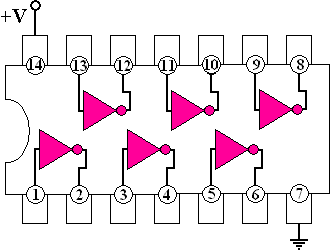
\includegraphics[width=110mm]{imageSources/hexInverter.png}
  
  \captionof{figure}{74HC04 Hex Inverter} 
  \label{hexInverter}
\end{minipage}

The servo used is the Hitec HS-55 who's datasheet can be found here. This is a very small servo that is controlled using pulse width control. It requires at least 4.8 volts of power, so it must be powered by the source, the AT90 only produces 3.3 volts.


  \begin{minipage}{6.5in}
    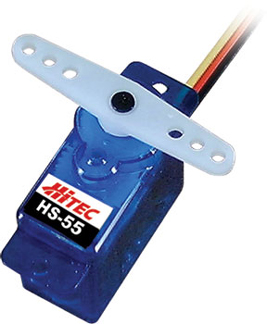
\includegraphics[width=90mm]{imageSources/servo.png}
  \centering
  \captionof{figure}{Hitec HS-55 Servo} 
  \label{servo}
\end{minipage}


\subsubsection{Joystick}
We used a traditional serial joystick. The joysticks port is a Male version of the above diagram. We then took a male connector and wired the ports that we wanted. X, Y ground and power. 


  \begin{minipage}{6.5in}
    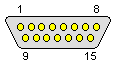
\includegraphics[width=90mm]{imageSources/joystick.png}
    \captionof{figure}{Joystick Pinout} 
  \label{joystick}
\end{minipage}


Table \ref{joystickPinout} describes the functions of each pin of the
joystick:

\begin{minipage}{6.5in}
\captionof{table}{The joystick pinout}
\begin{center}
\begin{tabular}{ c c c } 
  Pin Number & Signal Name & Description \\
  \hline
 1 & +5V & Power \\
 2 & Right Button 1 & Button 1 \\
 3 & X-Position 1 & Joystick 1 X-Coordinate \\
 4 & Signal GND & Ground \\
 5 & Signal GND & Ground \\
 6 & Y-Position 1 & Joystick 1 Y-Coordinate \\
 7 & Left Button 1 & Button 2 \\
 8 & +5V & Power \\
 9 & +5V & Power \\
 10 & Right Button 2 & Button 4/Joystick 2 Right button \\
 11 & X-Position 2 & Joystick 2 X-Coordinate \\
 12 & MIDI Out & MIDI Output \\
 13 & Y-Position 2 & Joystick 2 Y-Coordinate \\
 14 & Left Button 2 & Button 3/Joystick 2 Left button \\
 15 & MIDI In & MIDI Input \\
\end{tabular}
\label{joystickPinout}
\end{center}
\end{minipage}

\subsubsection{UART}
For testing purposes, when we wanted two UART readings, we used a windows machine and serial UART. For serial UART connections, the ADM33L chip is used to convert the signal. This chip is intended for use with transmitting and receiving devices. We use it for RS-232 transmission of data from the AT90 to a serial connection on a HyperTerminal running on the computer. This chip has an on board voltage converter to allow it to run from a single 5 volt power supply. 

  \begin{minipage}{6.5in}
    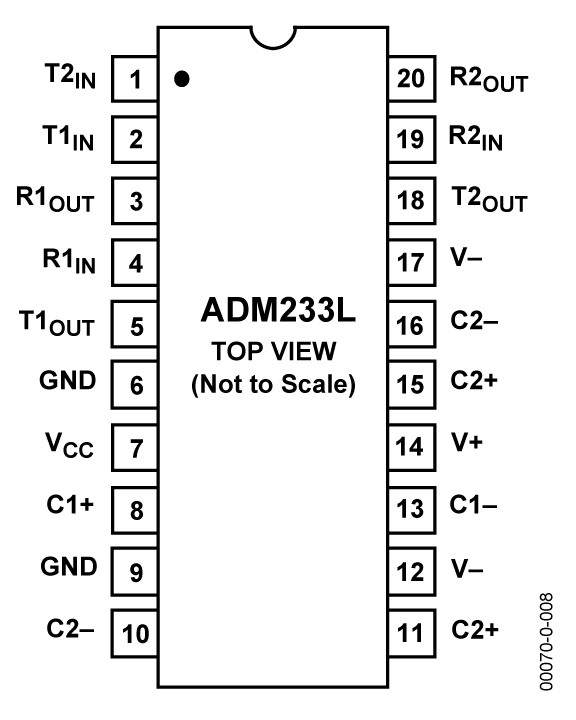
\includegraphics[width=90mm]{imageSources/serialUART.png}
  \centering
  \captionof{figure}{Serial UART Schematic} 
  \label{serialUART}
\end{minipage}


We are using USB to UART Bridge - FT232RL. This bridge is able to be connected directly to the board with out the use of an extra chip. This chip is powered using the 3.3 volts of power provided by the connection to the computer. 


  \begin{minipage}{6.5in}
    \centering
    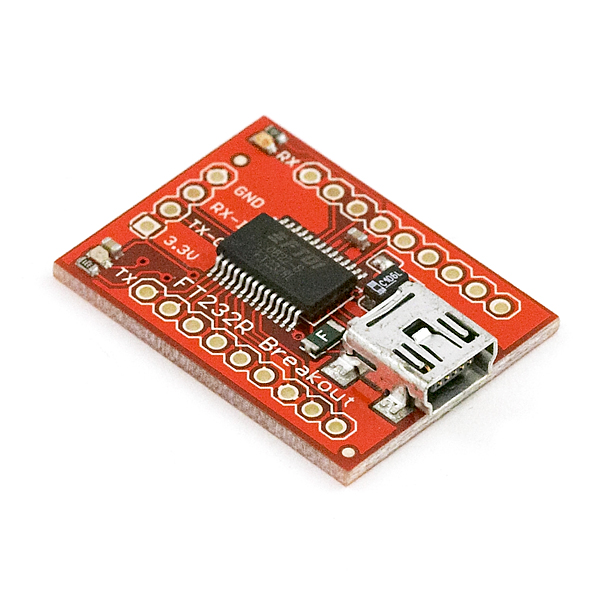
\includegraphics[width=90mm, height= 70mm]{imageSources/usbUART.png}
  \captionof{figure}{USB UART} 
  \label{usbUART}
\end{minipage}

\subsubsection{Sonar}
This sonar is capable of both long and short distance readings. It can tell if there is an object present from 0-254 inches, and gives distance information for objects 6-254 inches. This sonar has ground, VCC, enable and three different pins to read information(PWM, analog, digital). We chose to use the PWM.  When the enable pin is pulled high then the sonar will send out signals and listen.  The datasheet for the Max Sonar EZ1 can be found here.

  \begin{minipage}{6.5in}
    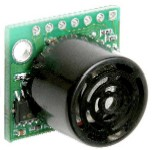
\includegraphics[width=70mm, height= 70mm]{imageSources/sonar.png}
  \centering
  \captionof{figure}{Max Sonar EZ1} 
  \label{sonar}
\end{minipage}

\subsection{Connections and Interface Design}
This section describes the connections among the various components, as well as other factors relating to the design of the electronic configurations used.  

\subsubsection{Power}
To power many of the components (Motors, Sonar, RS-232 Uart) we required more than the 3.3 volts of power than the USB provided. For this we needed to get power from the wall. Direct power from the wall reads between 9-12 Volts (our cords were supposed to produce 12, but they often had fluctuating readings).  This power needed to be minimized to a managable 5 volts.  The image below shows the setup to do this conversion.

  \begin{minipage}{6.5in}
    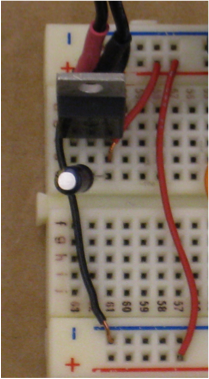
\includegraphics[scale=0.75]{imageSources/power12to5.png}
  \centering
  \captionof{figure}{Conversion from 12 to 5 volts} 
  \label{power12to5}
\end{minipage}

\subsubsection{Radio Connections}
\label{radioconn}


There is one radio present on each of the boards. The radio on the base station board sends the information regarding the position of the joystick and then prints the information it receives from the hover station.  The radio on the hovercraft sends information regarding the output of the motor and the sonar reading and receives information to change the position of the two motors.

All of the wires from the radio go to port E. The Radio ground pin must also be connected to the ground on the bread board. As modeled in the above diagram, the pin layout for the radios are as follows:

  \begin{minipage}{6.5in}
  \centering
    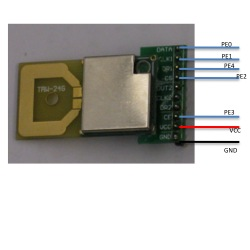
\includegraphics[width=90mm]{imageSources/radioConnect.png}
  
  \captionof{figure}{Radio Wiring Layout} 
  \label{radioConnect}
\end{minipage}

\subsubsection{Motor Connections}
An H-bridge is used to  control a motor that you want to spin in two different directions. Below is a diagram behind the theory of an H-Bridge taken from Wikipedia. An h-bridge is composed of a power source, four switches and a motor. The switches can all be in one of two positions, open or closed. There are only two different positions that the entire h-bridge can be in (shown in the diagram below). On the left, the lower left and upper right switches are open. this makes a circuit that goes through the motor from left to right, this will make the motor spin one way.  In the right diagram the other two switches are open, this makes the current flow through the motor from right to left, making the motor spin in the opposite direction.

  \begin{minipage}{6.5in}
    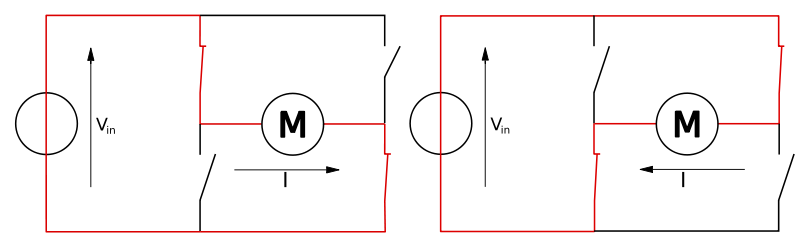
\includegraphics[width=90mm]{imageSources/hBridgeConnect1.png}
  \centering
  \captionof{figure}{Diagram of the H-bridge for a DC Motor} 
  \label{hBridgeConnect1}
\end{minipage}


  \begin{center}
    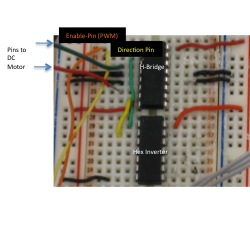
\includegraphics[width=90mm]{imageSources/hBridgeConnect2.png}
  \end{center}
  \captionof{figure}{Layout of the H-bridge} 
  \label{hBridgeConnect2}


In the above diagram, the orange enable pin is attached to OCR0A. This pin outputs the PWM signal needed to control the speed of the motor.  The yellow direction pin is connected to pin C1. This pin is either pulled HIGH or LOW which changes the position of the switches in the H-bridge.

\subsubsection{Joystick Connections}

For this project we are using an analog joystick. This means that  the joystick reads off many different readings to calculate its position. Details of how the conversion from analog to digital are outlined in the implementation section.

Pin 3, the x value, is wired to the first pin of PORT F (PINF1). The y value is connected to the second pin of PORT F (PINF2). Lastly, the second Y value is wired to the forth pin of PORT F (PINF4).

  \begin{minipage}{6.5in}
    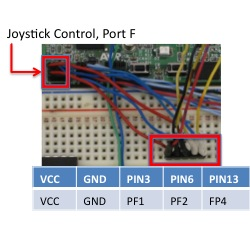
\includegraphics[width=90mm]{imageSources/joystickConnect.png}
  \centering
  \captionof{figure}{Joystick Connection: Pin Layout} 
  \label{joystickConnect}
\end{minipage}

\subsubsection{UART Connections}
The ADM233L connects to both the serial cable, and the AT90. 


  \begin{minipage}{6.5in}
    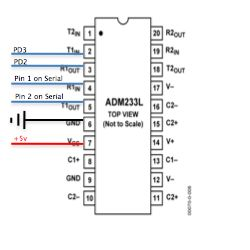
\includegraphics[width=90mm]{imageSources/uartConnect1.png}
  \centering
  \captionof{figure}{UART Pin Layout for ADM233L} 
  \label{uartConnect1}
\end{minipage}


  \begin{minipage}{6.5in}
    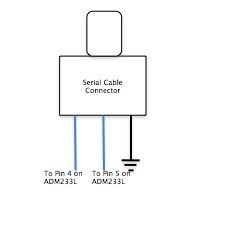
\includegraphics[width=90mm]{imageSources/uartConnect2.png}
  \centering
  \captionof{figure}{UART Pin Layout For Serial} 
  \label{uartConnect2}
\end{minipage}


  \begin{minipage}{6.5in}
    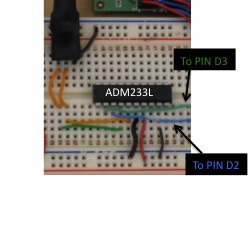
\includegraphics[width=90mm]{imageSources/uartConnect3.png}
  \centering
  \captionof{figure}{UART Wiring Layout} 
  \label{uartConnect3}
\end{minipage}

The above image is a picture of the UART layout of the board. In this picture, you can also see the layout for the power supply.

The USB UART is connected to the board on the same pins as the serial UART.  This chip has three output wires.  GND, TX-O, RX- I. This chip connects directly to the board. TX-O connects to PD2 and TX-I connects to PD3, the GND output connects directly to ground on the AT90.

\subsubsection{Servo Connections}
The servo motor requires 5 volts of power, to be connected to ground and a pwm signal to run. To generate the PWM signal a 16 bit timer must be enabled and the input wire on the servo must be connected to the proper output compare. For this component we used timer 1 and connected the servo to OC.1B which is located on PB6.

\subsubsection{Sonar Connections}
The sonar must be connected to two pins on the AT90 and to ground and power on the bread board. We decided to calculate the distance using PWM even though we could have used a few methods. (See sonar implementation for details on the conversion.)  For this the sonar needed to be attached to a pin on the board to be triggered when the input goes high. This pin also needs to be associated with a timer. We chose to use timer three for our sonar, and Input Capture Register (ICP3) to read the input which is located on port C7. The sonar will also only fire when the RX pin reads high. So we connected the RX pin to PC6 and then set that pin either high or low.

  \begin{minipage}{6.5in}
    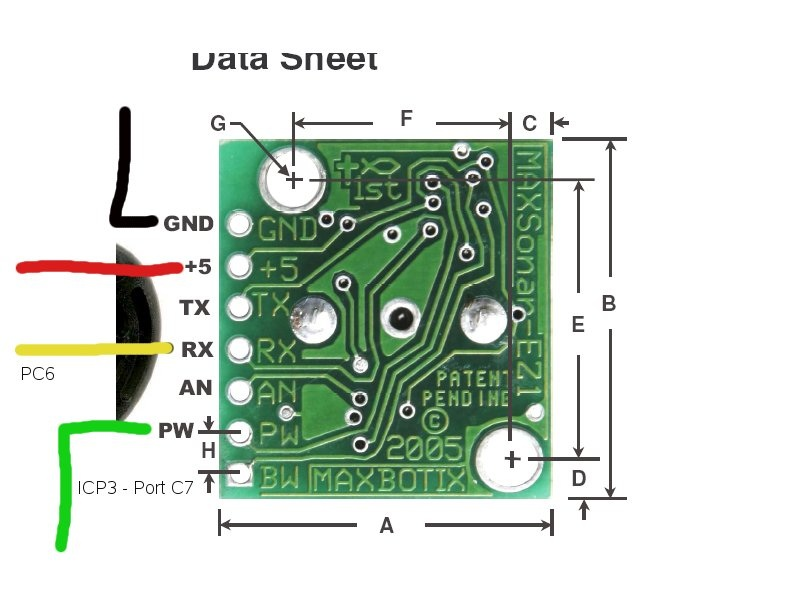
\includegraphics[width=90mm]{imageSources/sonarConnect.png}
  \centering
  \captionof{figure}{Sonar Wiring Layout} 
  \label{sonarConnect}
  \end{minipage}



\clearpage
\section{Hovercraft Design and Construction}
Research on various aspects of hovercraft design, mechanics and physics first principles, as well as input from the TA and the design decisions of our peers, led us to our own hovercraft design. This document first describes the information we uncovered about the mechanics of a hovercraft, then proceeds by describing our design and summarizing our final product.

\subsection{Hovercraft Mechanics}
The hovercraft is able to move freely due to the minimum amount of friction between the vehicle and the ground. The chamber of air between the craft and ground, called the plenum chamber, is formed by the body of the hovercraft and a skirt. The air flowing into the plenum chamber forms a ring which keeps the external lower pressure out, ensuring the persistence of the internal air cushion. The amount of air entering the plenum chamber must be at least be equal to the amount of air that escapes underneath the skirt in order to keep the craft afloat. Further, it is incorrect to assume that air will escape evenly around the skirt’s perimeter. As more air is blown into the plenum chamber, the pressure of the air on the inside becomes higher than that on the outside, creating an upward force that lifts the hovercraft. When this upward pressure exactly matches the downward force of gravity, the desired floating effect is achieved. \cite{CambridgeJournals:370274} \cite{831309}

\subsubsection{Steering}
Different approaches have been taken to steer the craft. Larger hovercrafts typically employ a large propeller at the rear to drive the vehicle forward. Rudders are used for steering. Another option, usually seen in smaller hovercrafts, is to tilt the base, affecting the plenum chamber underneath. This results in a change in direction because a drag is created on one side, creating a pivot point.


  \begin{center}
    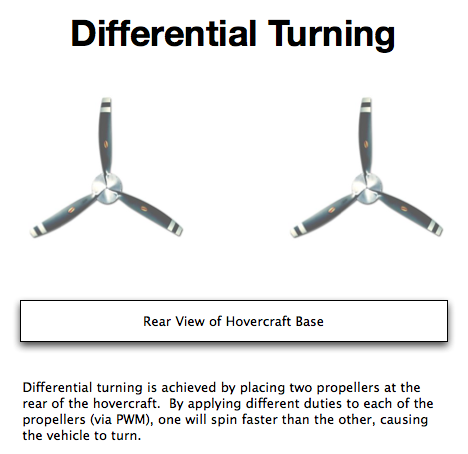
\includegraphics[width=85mm]{imageSources/differentialTurning.png}
  \end{center}
  \captionof{figure}{Differential Turning} 
  \label{differentialTurning}


Instead of using 2 fans on the craft (one for filling the plenum chamber and one for forward thrust), a single propeller may be used for both functions. A fraction of the air intake is directed into the inner chamber to lift the craft, while the remaining air flow is forced behind the craft, creating thrust.


  \begin{center}
    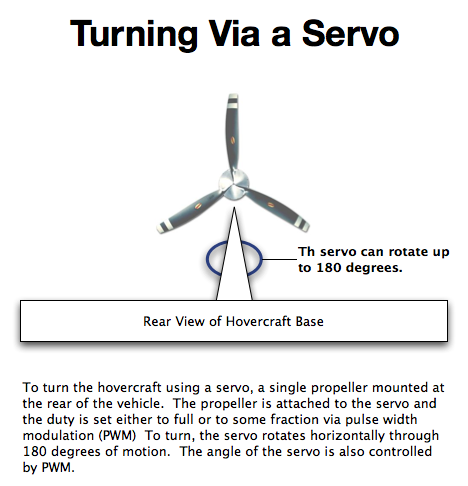
\includegraphics[width=85mm]{imageSources/servoTurning.png}
  \end{center}
  \captionof{figure}{Servo Turning} 
  \label{servoTurning}


Steering may further be affected by either differential turning or though the use of a servo motor. The former approach commonly employs two thrust sources on either side of the vehicle. By altering the thrust of either motor (for example with pulse width modulation), one motor will be more powerful than the other, causing the craft to turn. The latter approach sees a propeller mounted to a servo motor. As the servo rotates through its 180 degree range, the thrust of the propeller is directed in a specific direction, also causing the craft to turn.

\subsubsection{Skirt}
An advancement in the development of the skirt is known as the Double-Walled Flexible Skirt, or more commonly the “Big Skirt”. The design came about in the 1960’s by McReary. The idea was to inflate the outer skirt to allow the craft to move more freely over rough terrain and choppy water.

In general, the purpose of the skirt is to increase the overall surface area of the vehicle. By spreading the weight of the craft over a lager area, the pressure required to counteract this downward pressure is reduced. A common analogy is that of stepping on a single nail as opposed to lying on a bed of nails. Applying one’s entire weight on the small surface area of a single nail will surely result in a painful experience. However, by spreading one’s weight over the combined surface area of many nails, the pressure on any single point is reduced to the point where any particular nail cannot cause harm.

\subsection{Ground Effect}
Ground effect refers to the collection of aerodynamic effects felt by aircraft when flying in close proximity to the ground. If the hovercraft has too much lift, it is likely that it may well feel the effects of such a phenomenon.


  \begin{center}
    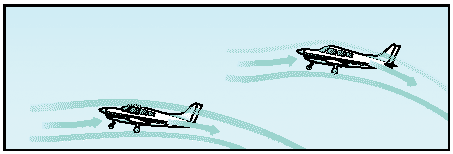
\includegraphics[width=85mm]{imageSources/groundEffect.png}
  \end{center}
  \captionof{figure}{Ground Effect Airflow} 
  \label{groundEffect}

One of the most prominent is the Wing-In-Ground effect, whereby the aircraft experiences reduced amounts of drag when flying at an altitude less than the length of its wingspan. Though the physics are somewhat complicated and beyond the scope of this report, the result is an increase in speed and lift when flying in ground effect. Ground effect is more significant for lighter aircraft than for heavier aircraft. Ground effect also has implications for rotary aircraft like helicopters. They require less energy to remain air bourn while in ground effect.

\subsection{Vortex Ring Effect}
Another interesting property of propellers, such as those used in Helicopters, is Vortex Ring effect. As helicopter blades spin, they direct air downwards, creating lift. Sometimes this air may recycle, looping around and reentering the blades. This can have a drastic effect on lift.

\begin{figure}[h]
  \begin{center}
    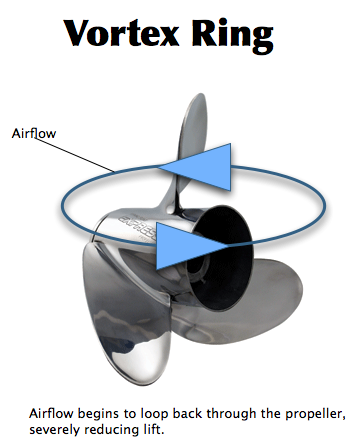
\includegraphics[width=85mm]{imageSources/vortexRing.png}
  \end{center}
  \caption{Vortex Ring Effect} 
  \label{vortexRing}
\end{figure}

\subsection{Design Schematics}

The following figures show the top, side, front and rear views for the vehicle:

\begin{figure}[h]
  \begin{center}
    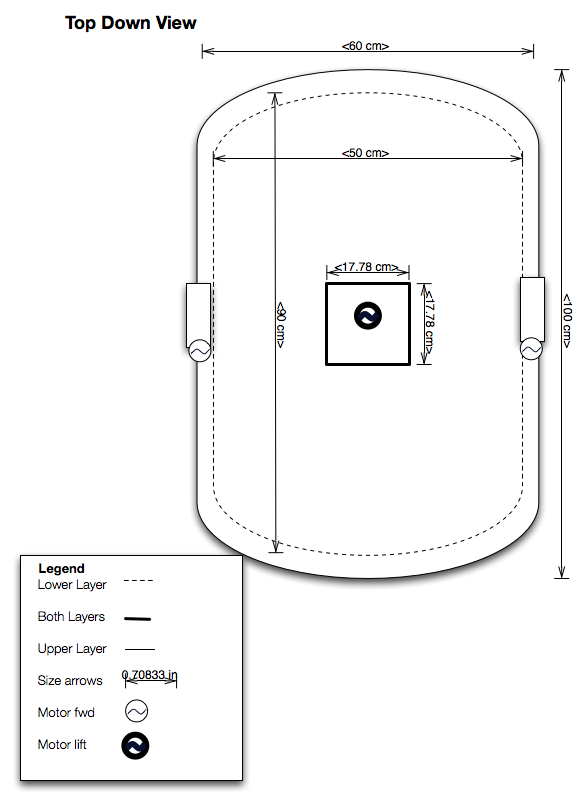
\includegraphics[width=85mm]{imageSources/topDownView.png}
  \end{center}
  \caption{Hovercraft: Top Down View} 
  \label{topDownView}
\end{figure}

The first design consisted of a rounded front, straight sides and a straight back. However, since the front and back were not symmetric, we concluded that the rear of the craft should be rounded to match the front. This symmetric design better distributes the underlying air cushion to all parts of the vehicle.

  \begin{center}
    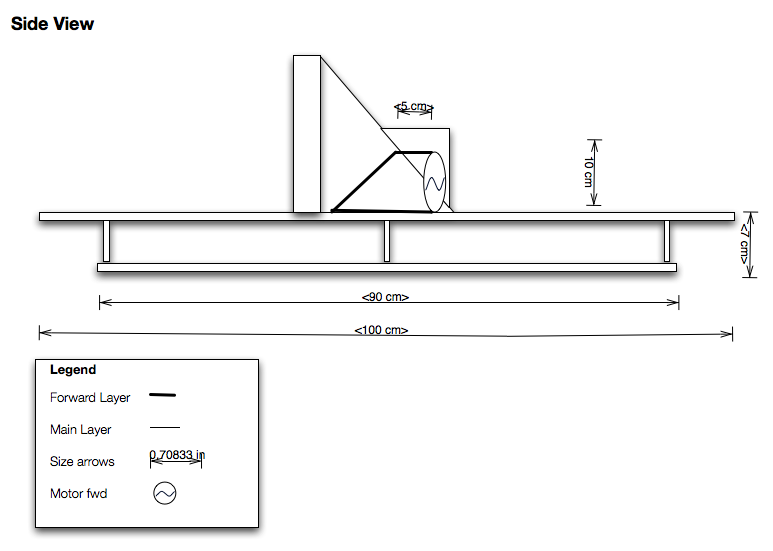
\includegraphics[width=85mm]{imageSources/sideView.png}
  \end{center}
  \caption{Hovercraft: Side View} 
  \label{sideView}

The plenum chamber receives air from a single propeller mounted in the middle of the chasis. The middle propeller is housed by a triangular container. Initially the container was completely open on the side where the propeller draws air from. We realized that too much air was escaping from this hole and a cover with a circular cut-out was fitted over the opening. The cut-out better fit the diameter of the fan, resulting in minimal air escaping from the opening.


  \begin{center}
    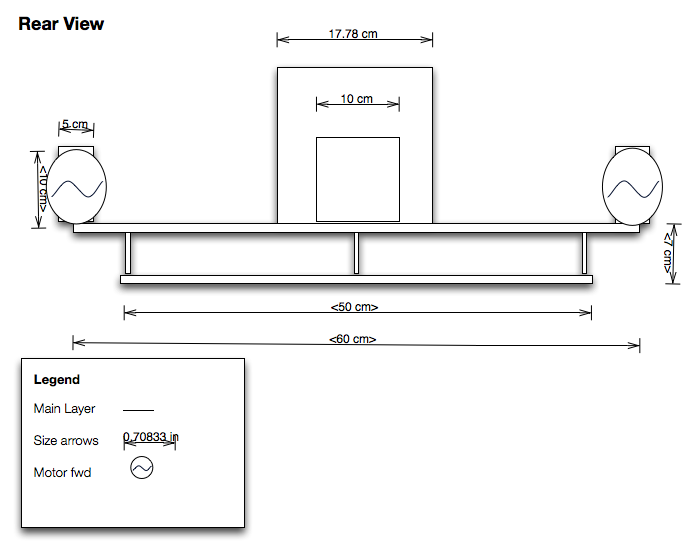
\includegraphics[width=85mm]{imageSources/rearView.png}
  \end{center}
  \caption{Hovercraft: Rear View} 
  \label{rearView}


The electronic components are mounted at the rear of the hovercraft. This facilitates making connections from the breadboard to the nearby DC Motors, servo motor, and sonars. The combined mass of all the components added a significant force to the rear of the chasis. To counter this, we placed counter weights on the front of the body.

\begin{figure}[h]
  \begin{center}
    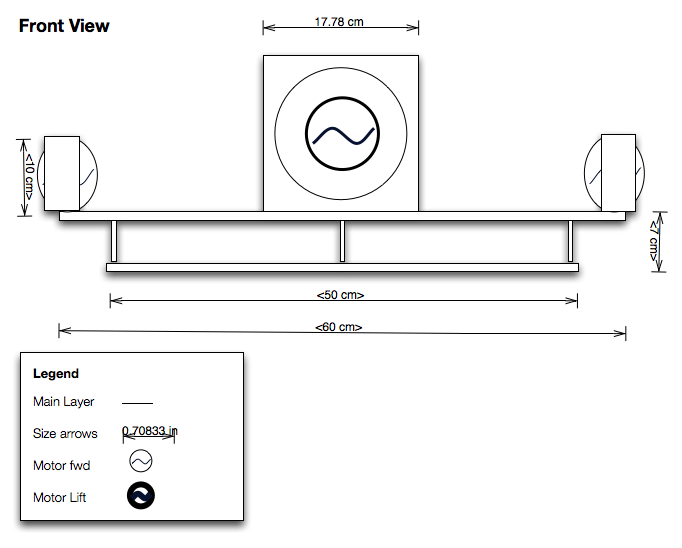
\includegraphics[width=85mm]{imageSources/frontView.png}
  \end{center}
  \caption{Hovercraft: Front View} 
  \label{frontView}
\end{figure}

\subsection{Design Constraints}
The following constraints were issues that needed to be met by the resulting hovercraft design.

\subsubsection{Payload Weight}
In order for the hovercraft to stay afloat, the internal air pressure must counter external forces placed on the surface of the vehicle by both gravity and the mass of the components. The following table describes the components and their masses:

\begin{table}
\caption{Weight of Hovercraft Components}
\begin{center}
\begin{tabular}{ c c c}
  Component & Quantity & Weight (grams) \\
  \hline
	Battery  &	2 & 	50 \\
	Breadboard &	1 &	45 \\
	Microcontroller &	1 &	15 \\
	Radio &	1 &	9 \\
	Sonar &	3 &	5 \\
	DC Motor (large) &	1 &	83 \\
	Servo Motor &	1 &	4 \\
	H-bridge &	1 &	6 \\
	DC Motor (small) &	2 &	25 \\
	Total &	-- &	329 \\
\end{tabular}
\end{center}
\label{restingTable}
\end{table}

\subsection{Rigidity}
The hovercraft body is made from two thin sheets of styrofoam separated by 12 styrofoam spacers 1'' thick. This has proven to be a very strong design, easily capable of supporting the payload of the electronics. In fact, we distributed additional weight evenly across the body and found that the hovercraft could support at least 1 kg.

\begin{figure}[h]
  \begin{center}
    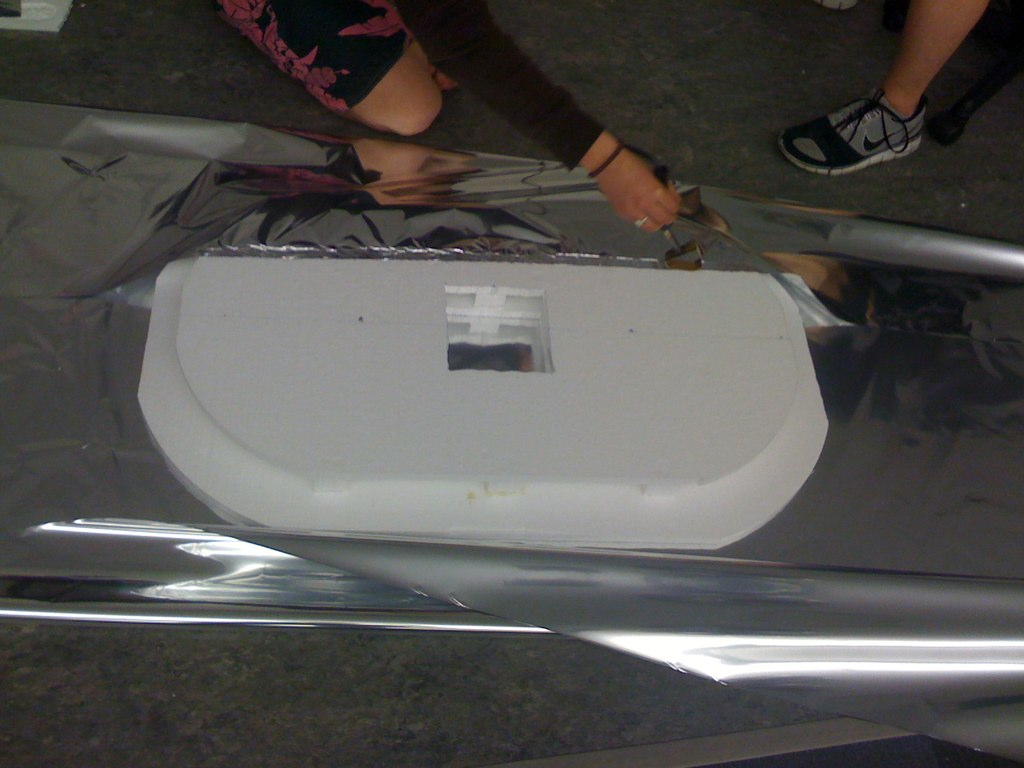
\includegraphics[width=85mm]{imageSources/rigidity1.png}
  \end{center}
  \caption{Rigidity of Hovercraft I} 
  \label{rigidity1}
\end{figure}

\begin{figure}[h]
  \begin{center}
    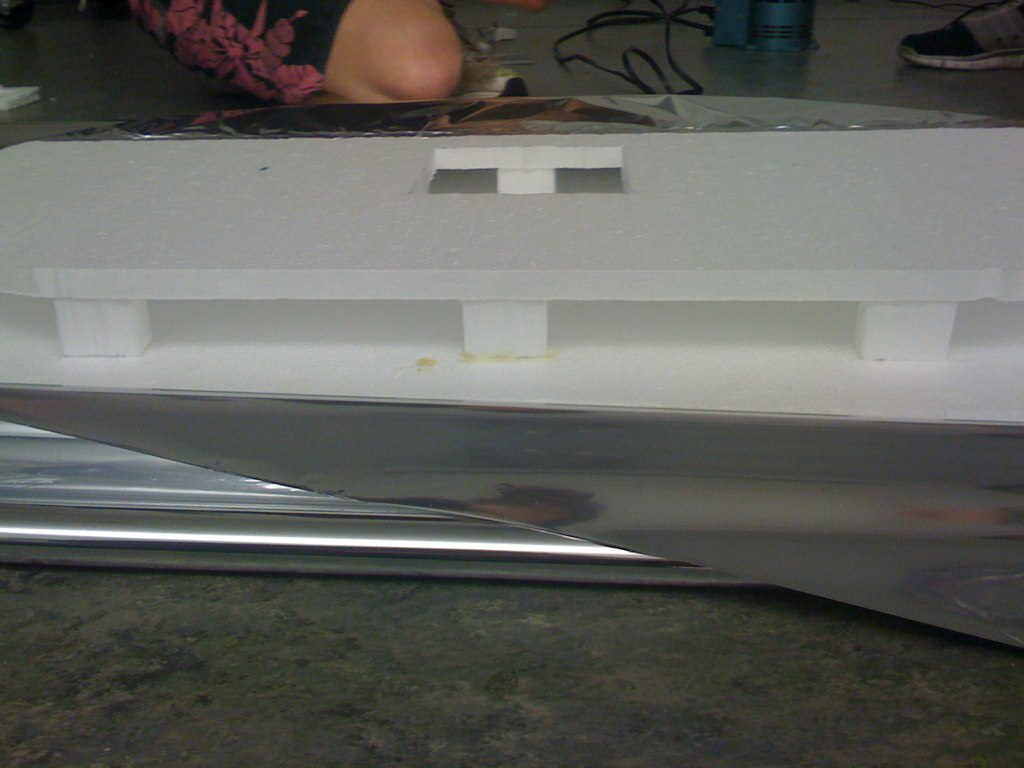
\includegraphics[width=85mm]{imageSources/rigidity2.png}
  \end{center}
  \caption{Rigidity of Hovercraft II} 
  \label{rigidity2}
\end{figure}

An inflatable skirt made of mylar surrounds the body. Mylar is a polyester film often used in flexible packaging for food, as an insulating material, and for solar reflection. Once inflated, the skirt serves two purposes. First, because it expands to over two inches, it provides additional surface area, reducing the overall pressure at any given point on the body. Second, the skirt acts as a flexible and damage resistant bumper, protecting the body from nearby objects during testing. We used two different mediums to connect the skirt to the styrofoam body. First we adhered the mylar to the styrofoam using hot glue, we then went around the perimeter with a hot iron to melt the mylar, the glue and the styrofoam together.

\begin{figure}[h]
  \begin{center}
    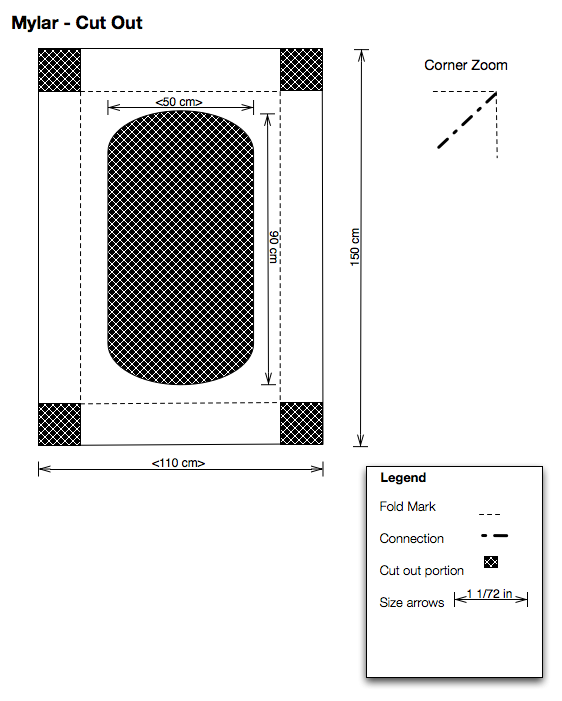
\includegraphics[width=85mm]{imageSources/mylarSchematic.png}
  \end{center}
  \caption{Schematic of the Mylar skirt} 
  \label{mylarSchematic}
\end{figure}

After the styrofoam chasis was built, we then procdeded to construct the skirt. The first attempt at constructing the mylar skirt was not successful. Lack of foresight resulted in a skirt that was too baggy in some areas, while exposing too many holes in others. The first time that we attached the mylar, when we were connecting the corners, we used clear packing tape, and simply folded the corners together. The second attempt was much more calculated and pragmatic. When connecting the corners of the second skirt, we methodically folded the edges in, then removed the square that was not attached (see Mylar-Cutout diagram). After this we made the connection using the hot iron to glue the seam together. The resulting skirt was much more evenly distributed and provided reasonably uniform inflation around the entire body. That said, the hovercraft still managed to move about when it was supposed to be idle. We addressed this issue by placing weights on the body to counteract the uneven escape of air on one side.

\subsubsection{Lift}
The decision to use a single, vertically mounted propeller to feed air into the plenum chamber was in direct response to the problem of rotational torque plaguing horizontally mounted propellers. In a horizontal design, the rotation of the blades applies an overall torque on the hovercraft causing it to spin. Dealing with this force is a burden. One approach is to install a second horizontal propeller which spins in the opposite direction. The opposite spin of the two motors cancels any directional torque felt by the craft. We chose to avoid this problem entirely by mounting a single motor vertically in the middle of the body. A container built over the propeller captures the incoming air and forces into the plenum chamber.

\begin{figure}[h]
  \begin{center}
    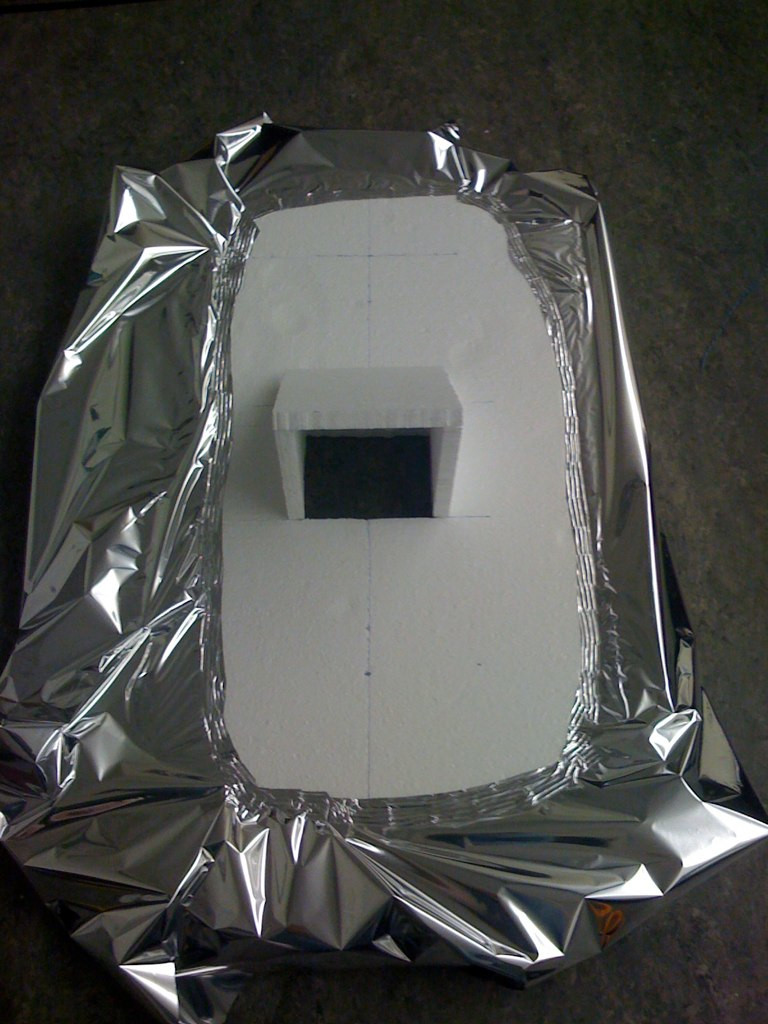
\includegraphics[width=85mm]{imageSources/lift1.png}
  \end{center}
  \caption{Hovercraft Lift I} 
  \label{lif1}
\end{figure}

\begin{figure}[h]
  \begin{center}
    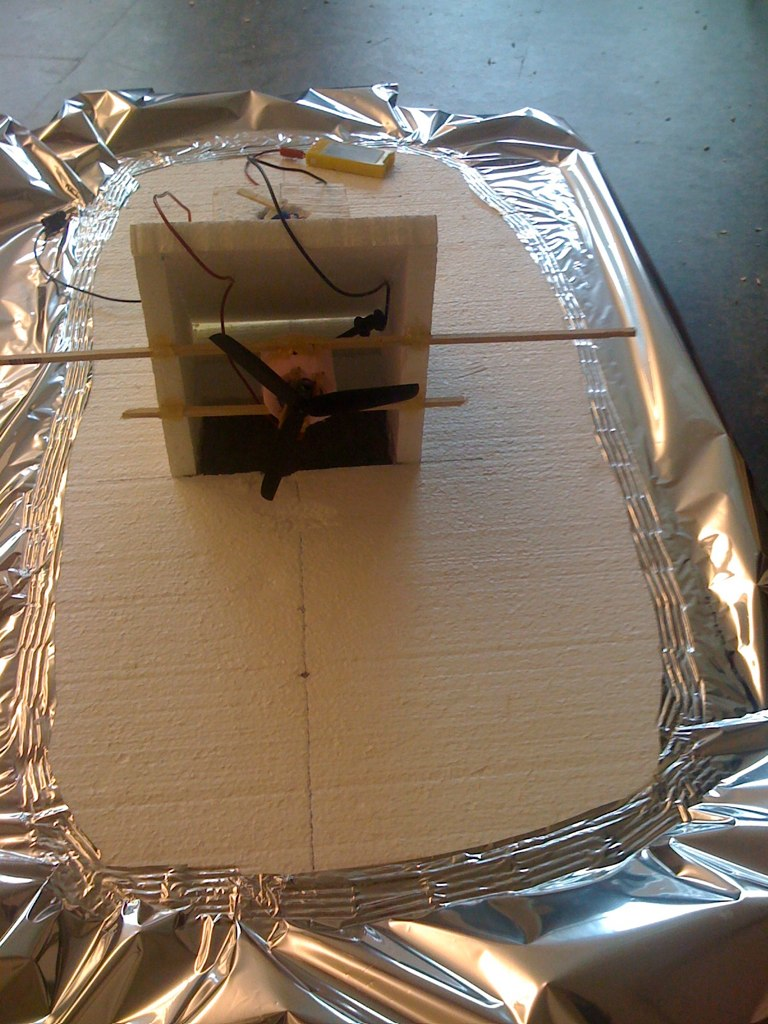
\includegraphics[width=85mm]{imageSources/lift2.png}
  \end{center}
  \caption{Hovercraft Lift II} 
  \label{lift2}
\end{figure}

To avoid ground effect, we applied full power to the lift propeller. Next, we methodically added weight to the body such that the hovercraft moved freely along the ground, but was not vastly overpowered by the fan. Keeping the vehicle as close as possible to the ground allows for the most control over the hovercraft's direction.

\subsubsection{Thrust and Control}

The following two figures show the first design we had chosen to provide the vehicle with thrust. The two differential motors were mounted at the rear, and were spaced fairly close together.

\begin{figure}[h]
  \begin{center}
    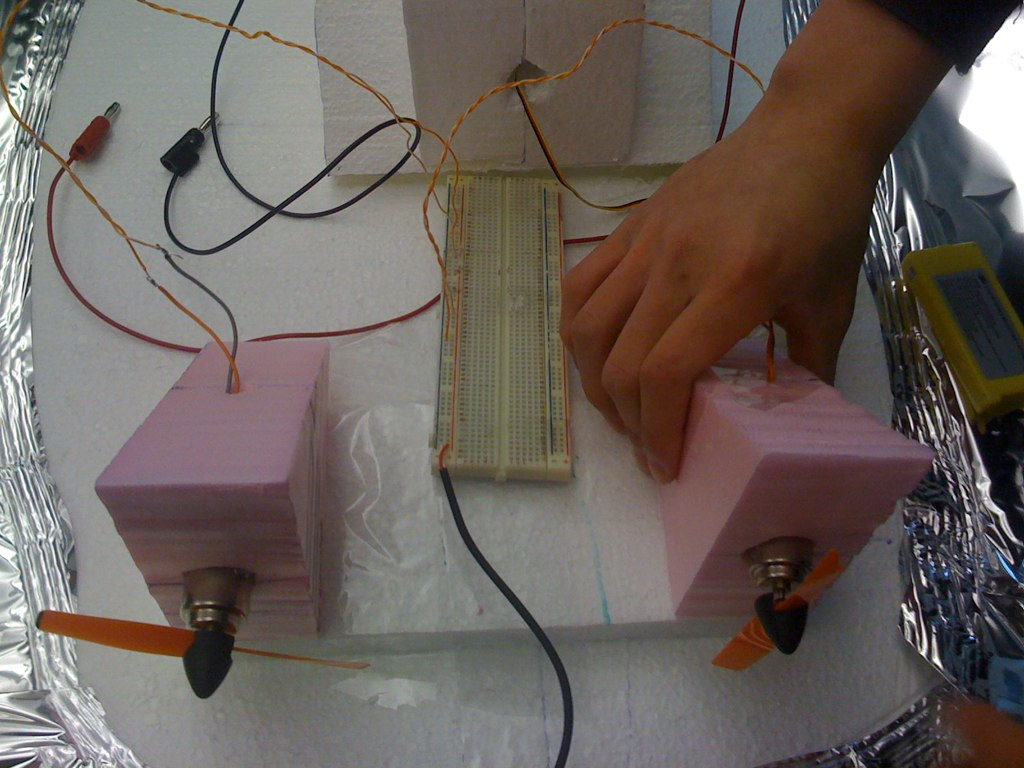
\includegraphics[width=85mm]{imageSources/thrustControl1.png}
  \end{center}
  \caption{Hovercraft Thrust and Control I} 
  \label{thrustControl1}
\end{figure}

\begin{figure}[h]
  \begin{center}
    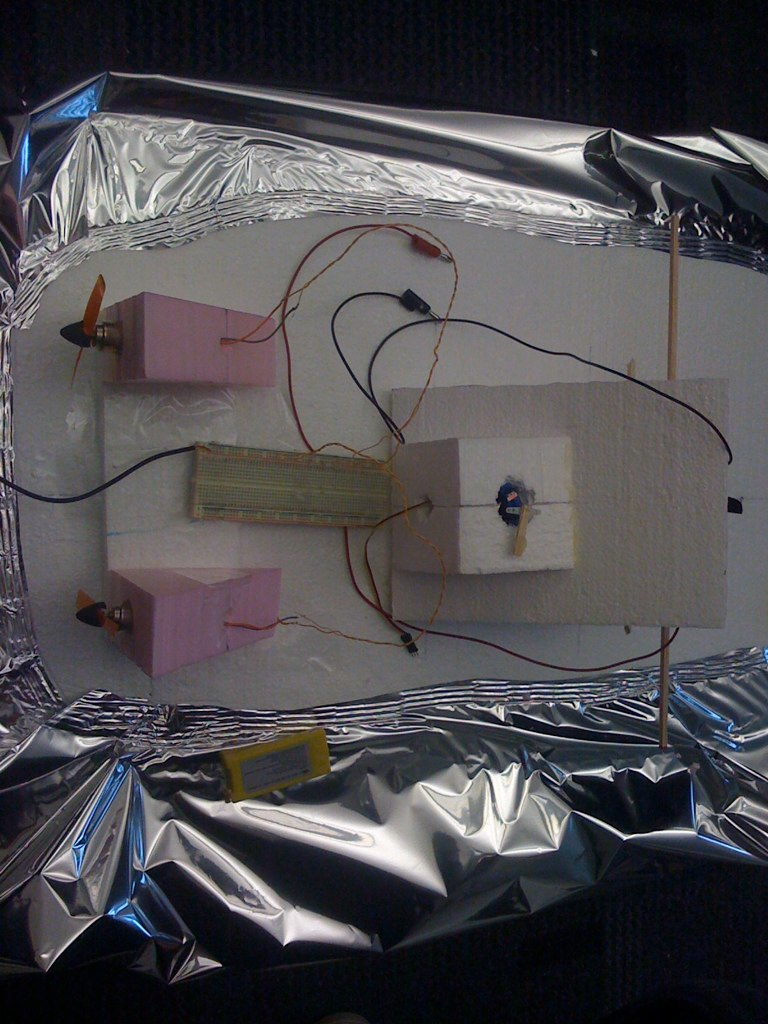
\includegraphics[width=85mm]{imageSources/thrustControl2.png}
  \end{center}
  \caption{Hovercraft Thrust and Control II} 
  \label{thrustControl2}
\end{figure}

We decided to change this design. By placing the motors as far apart as possible, maximum torque could be achieved. The analogy is as follows. Consider the act of opening a door. It is much easier to open a door if you push on the edge furthest from the hinges, because you can generate much more torque. The same goes for our hovercraft. Ideally the centre of rotation (the hinge) is in the centre of the hovercraft. By placing the motors as far away from this centre, we will create the most rotational torque and the craft will be easily controlled \cite{831309}.

\subsection{Design Problems and Future Considerations}
The following subsections describe the most challenging problems we encountered as the hovercrafts took shape.  

\subsubsection{Shape}
Our hovercraft is oval-shaped with a length to width ratio of 3:2. The first problem we encountered with this shape was that it was hard to evenly wrap our mylar around the soft corners. The mylar creased around the corners, and stuck out unevenly, often hanging down enough to provide friction for the hovercraft, creating a pivot point when we tried to move the hovercraft around. We had to make extra cuts, and then iron and glue the corners to prevent this. A hovercraft with sharper edges may take significantly less mylar tuning, and we haven't found speed to be a major issue, so the fact that square edges may reduce the aerodynamics of the hovercraft may not be as significant an issue as we thought.

\subsubsection{Weight Distribution}
Our fan blows air parallel to the ground, and we have a Styrofoam encasing around the fan directing the air down into the hovercraft base, with a single hole at the bottom of the hovercraft in the center. As mentioned above, we tried to seal the mylar around the edges of the hovercraft so that it was air-tight. We cut a Styrofoam circle that had a diameter just slightly bigger than that of the fan, and placed it even with the edge of the fan, in order to get the maximum possible amount of air intake, and prevent as little air as possible from escaping. Our fan motor is large, and is able to easily lift our hovercraft, and with this design we haven't come across any lift-related issues. The main problem we encountered having a single large fan is that it is being held up by the small square Styrofoam encasing, under 20cm in length. The fan makes up a significant portion of the overall weight of our hovercraft, and the weight distribution is all in the very center of the hovercraft. Because a large amount of the weight is in the very center, our hovercraft can easily tip, allowing air to flow out from the bottom of one side, resulting in the hovercraft gliding across the floor, or spinning.

\begin{center}
  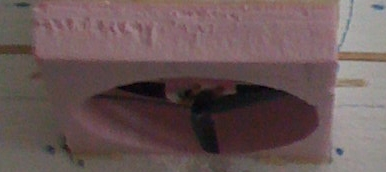
\includegraphics[width=85mm]{imageSources/weightDistro1.png}
\end{center}
\captionof{figure}{Weight Distribution I} 
\label{weightDistro1}

\begin{center}
  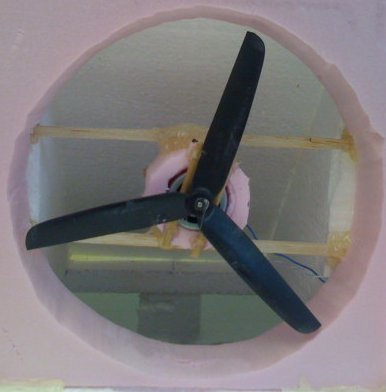
\includegraphics[width=85mm]{imageSources/weightDistro2.png}
\end{center}
\captionof{figure}{Weight Distribution II} 
\label{weightDistro2}

If the hovercraft moves around at all when just the lift fan is on, then it is extremely hard to control with the joystick. We initially hoped we could counterbalance this with software code, and shifted the power of the thrust motors on the side of the hovercraft accordingly. This took a lot of fine-tuning, and the hovercraft still was extremely hard to control, as air always seemed to be leaking from a different side, depending on the hovercraft's current movement direction and the forces exerted by the fans.

By placing weight around the edges of the hovercraft, we can greatly reduce the movement of the hovercraft when just the lift fan is on. The problem was that when enough weight was placed around the perimeter of the hovercraft that it remains motionless when the thrust motors are off, the fans had trouble moving the hovercraft forward or backward even at full power. As we took weight off, the motors could control the hovercraft more, but with less weight balancing the hovercraft, it again moves and spins uncontrollably.

\subsubsection{Turning Pivot}
We originally had our motors placed at the back end of our hovercraft, as shown in the image below. We found that the turning pivot of the hovercraft is directly inbetween where the two thrust motors are placed. With the turning pivot at the back end of the hovercraft, the turning radius of the center of the hovercraft is equal to about half of the hovercraft's length (~90cm), and it was a awkward to control the hovercraft correctly. 

\begin{center}
  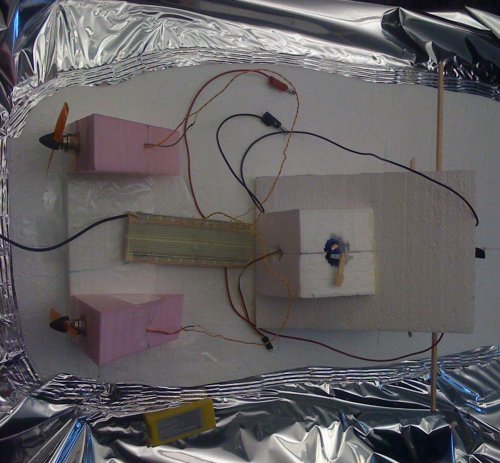
\includegraphics[width=85mm]{imageSources/turningPivot1.png}
\end{center}
\captionof{figure}{Turning Pivot I} 
\label{turningPivot1}

We shifted our thrust motors so that the fan blades were at the very center of our hovercraft. This allowed the hovercraft to have much tighter turns, and reduced our turning radius so that the hovercraft's pivot was right at the center of the hovercraft. We found controlling the hovercraft was much more intuitive this way.

\begin{center}
  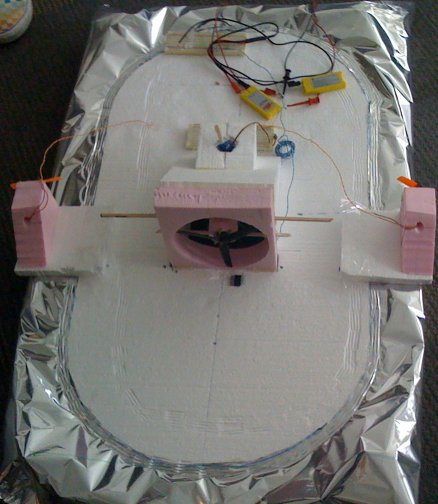
\includegraphics[width=85mm]{imageSources/turningPivot2.png}
\end{center}
\captionof{figure}{Turning Pivot II} 
\label{turningPivot2}

\subsubsection{H-bridge}
As mentioned above, one of the challenges that we encountered was that we were not getting enough power to our thrust motors. This lack of thrust was making it nearly impossible to accelerate in either direction. In the initial testing of our hovercraft design, we connected the thrusting motors directly to the 7 volt power source. In this experiment, the craft moved forward at a very quick speed over both the smooth linoleum floor and the carpet.

When testing our H-Bridge independently, it seemed like their was sufficient power being supplied to the thrust motors. Once we had the H-bridge and motors connected through the bread-board, along with the radio, and other components, the hovercraft hardly moved. The fans were moving much too slowly to accelerate our hovercraft. Our initial hypothesis was that there was not enough voltage being supplied to the H-Bridge. To solve this problem, we tried to connect an extra battery to one side of the bread-board to power the H-Bridge side, and another to control the other components on the bread-board. This solution did not seem to affect the thrust motors' power at all, as they still did not spin fast enough to accelerate our hovercraft.

After reading the documentation about the L293D H-Bridge, we found that it can only handle 1.5A maximum. At this point we tried a higher amperage H-Bridge. Again, when we wired the H-Bridge up independently, the motors spun very well, and significantly faster than with the previous L293D H-Bridge. Again, when we tested it with the rest of our components, the motors seemed to jitter, sometimes spinning as powerfully as we needed, but very irregularly. We thought this irregularity was due to a faulty H-Bridge, so we moved back to the L293D H-Bridges, that we were sure functioned correctly. As the 1.5A maximum was the limiting factor with the L293d H-Bridges, we decided to wire them in parallel. At 5 volts, this solution gave the fans almost enough power to control the hovercraft sufficiently. Unfortunately, when we used 7 volts, again the power shifted irregularly. Another problem was that we were using over 30 of the bread-boards 67 pins for our H-Bridges and Inverters alone, not leaving enough room for the other necessary components. We later found out that you can simply `piggy-back' the H-bridges, by soldering them on top of one another. This would solve the lack of pins issue. We have also since found out that the irregular power issues were caused because of the H-Bridges becoming too hot and shutting off. Attaching a heat-sink solves this problem, as we will discuss below, so two L293D H-Bridges may be a very viable option!

\begin{center}
  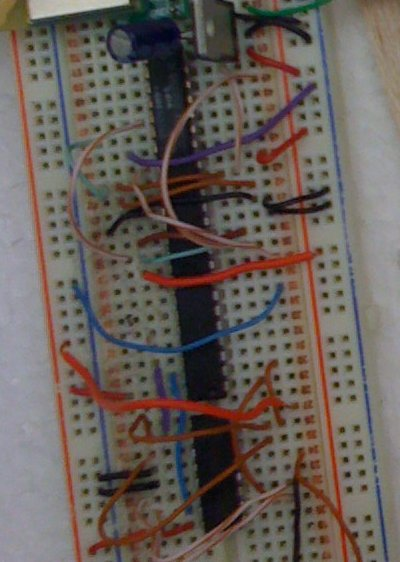
\includegraphics[width=85mm]{imageSources/designProblemsHBridge1.png}
\end{center}
\captionof{figure}{H-bridge Wiring Alternative I} 
\label{HbridgeWiring}

\begin{center}
  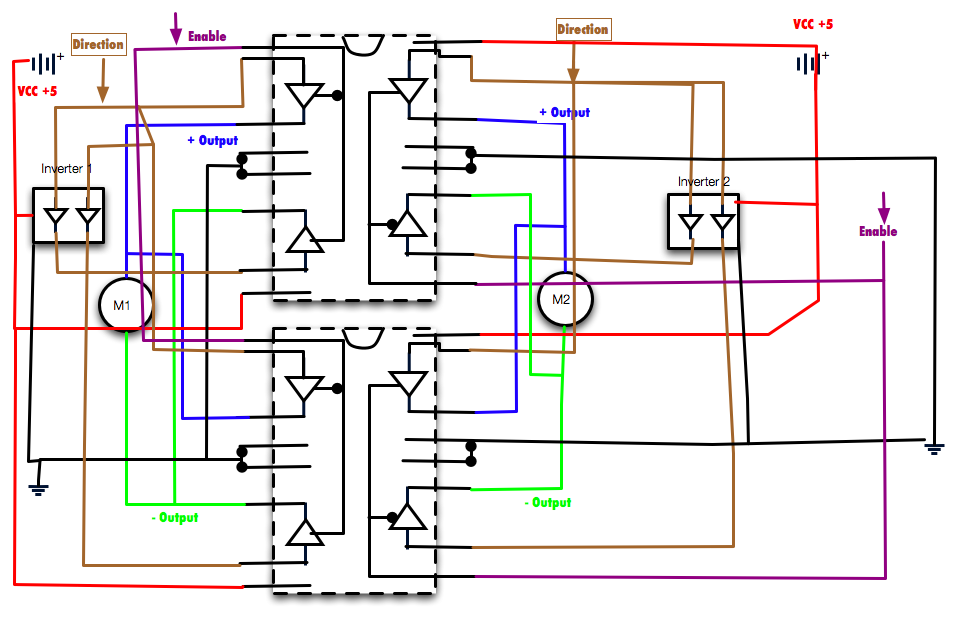
\includegraphics[width=85mm]{imageSources/designProblemsHBridge2.png}
\end{center}
\captionof{figure}{H-bridge Wiring Alternative II} 
\label{HbridgeWiring2}

At this point, we were supplied another high-amperage H-Bridge, so we went back to work on it. The new H-Bridge we were supplied also had an attached heat-sink. We were informed that the heat-sink would prevent the H-Bridge from becoming too hot and temporarily shutting off. With the heat-sink, the motors were getting enough power to successfully control the hovercraft, and the heat-sink prevented the irregular shifts in power caused by the H-Bridge shutting off.

\begin{center}
  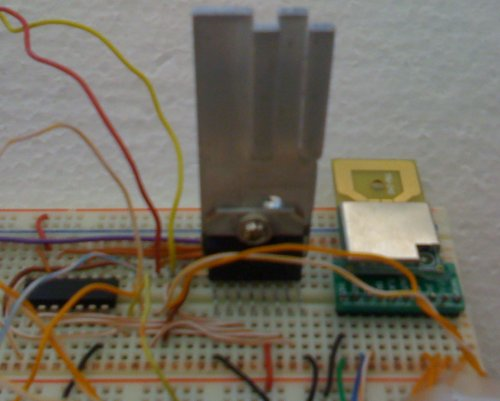
\includegraphics[width=85mm]{imageSources/designProblemsHBridgeHeatsink.png}
\end{center}
\captionof{figure}{H-bridge Heatsink} 
\label{HBridgeHeatsink}

\subsubsection{Joystick}
\label{sec:JoystickConst}
As the joystick we were supplied was seemed to produce different results every day that we tested it, and would not stay centered, it was very difficult to set-up our code to produce consistent results. We resorted to getting a new joystick that had not yet been modified to connect and work with the AT90. We took apart our new joystick, and found that it was currently using three potentiometers. One of the potentiometers was for the X position of the joystick, another was for the Y position, and the third was for the position of a dial on the base of the joystick. These potentiometers were connected so that the amount of current was determined by the position of the joystick, or the dial.

A potentiometer is a resistor with three terminals: a ground, an input, and an output (the wiper). There is a knob connected that can be spun, and as the knob is turned, the middle pin reads the voltage, and will output a reading that is the difference between ground, (zero) and the value of the input (in our case VCC).

\begin{center}
  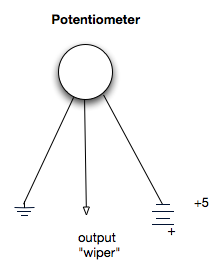
\includegraphics[width=85mm]{imageSources/joystickPotentiometer.png}
\end{center}
\captionof{figure}{Joystick Potentiometer} 
\label{joystickPotentiometer}

We decided to remove the potentiometer at the base of the joystick and simply control the hovercraft with the X- and Y-coordinates. We then were required to modify how the other two potentiometers were connected so that the amount of voltage was determined by the position of the joystick. To do this we grounded one side of the potentiometer, and connected power to the other. The middle connection was then connected through the serial port as output. Our current implementation outputs all three values at the base station, and sends them to the hovercraft, We may end up using the dial at the base of the joystick to control a ``side-stepping'' fan we could connect to the hovercraft that blows air perpendicular to the other fans. This would prevent the hovercraft from having to zig-zag down a hallway, as this fan could blow air toward the close wall to ``side-step'' the hovercraft away from the wall, without having to make an actual turn.

\begin{center}
  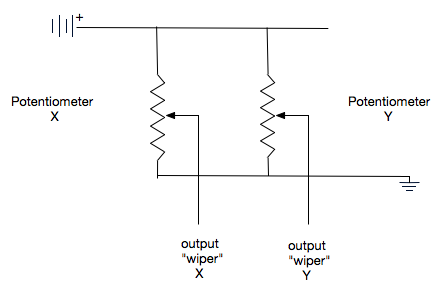
\includegraphics[width=85mm]{imageSources/potentiometerSchematic.png}
\end{center}
\captionof{figure}{Joystick Potentiometer Schematic} 
\label{potentiometerSchematic}

Once the casing was replaced on the joystick, the readings from the board, when the joystick was connected to 5 volts of regulated power, are displayed in the table below.

\begin{table}
\caption{Joystick Voltage for Direction}
\begin{center}
\begin{tabular}{ c c }
  Position & Reading (volts) \\
  \hline
  Forward & 3.76 \\
  Middle & 2.278 \\
  Backward & 0.633 \\
\end{tabular}
\end{center}
\label{voltagePotentiometerTable}
\end{table}

\subsubsection{Next Prototype}
In our next prototype, we will try and spread out the weight distribution of our center fan. This will reduce the amount of weight needed to place around the perimeter to balance the hovercraft, so the motors will be powerful enough to move the hovercraft. Now that we have our wiring completed, and are sure of the number of batteries, chips, fans, and bread-boards we will use, we can also plan a new design that takes into consideration their weights as well. Our large lift fan has always easily lifted our hovercraft, but we have found that it drains batteries quickly, our next design will also be a smaller hovercraft size, and therefore we will also use a smaller lift fan.

\clearpage
\section{PID Controller}
Upon completion of the vehicle body and electronic components, we ran into major weight balance issues. Since a hovercraft is practically floating on a thin layer of air, it is highly sensitive to weight imbalance. This imbalance causes the hovercraft to stray (yaw) off course, making it very difficult to control. Presented with such a situation, a PID controller can potentially correct the imbalance issues by having the hovercraft automatically compensate to the yaw produced by the imbalance.

\subsection{PID Controller Primer}
PID in PID controller stands for Proportional, Integral, Derivative. These three terms are used to define the behaviour of the controller. Each of them contributes to the final output of the controller, and different weights can be assigned to different terms. The weights selection process (tuning) is not an easy task. In a nutshell, a PID controller can output corrective actions based on the difference (error) between a set point (SP), the desired value, and a measured process variable (PV), the instantaneous value. A PID controller is a feedback control loop wherein the output of the controller is treated as an input of the same controller. The feedback allows the controller to intelligently adjust its output according to the error. 

\begin{figure}[h]
  \begin{center}
    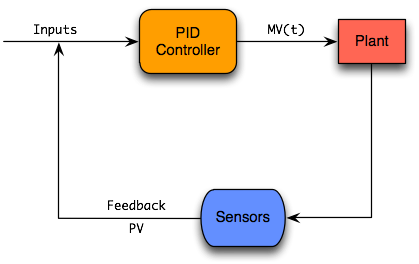
\includegraphics[width=85mm]{imageSources/pidcontroller.png}
  \end{center}
  \caption{A simple PID controller} 
  \label{pidController}
\end{figure}

The object being controlled by the PID controller is usually referred as the plant, as shown in the above diagram. Depending on the system, a plant can be a motor, servo, actuator, and etc. The plant is constantly monitored by some sensors in order for the PID controller to adjust its output based on the error.

\subsection{PID Terms}
As mentioned earlier, there are three terms that determine the behaviour of the PID controller. The calculated output or Manipulated Variable (MV) of the PID controller is the summation of all three terms. The formula can be written as: OOOOOOOOOOO INSERT MATH EQUATION HERE 00000000 where Kp, Kd, and Ki are the weight constants or the tuning parameters, and e is the error calculated by subtracting the set point(SP) by the process variable(PV) or SP - PV.

\subsubsection{Proportional Term}
The proportional term in the PID controller corresponds to how fast the controller reacts to error. Depending on the parameter Kp, the magnitude of the proportional term will either amplify or diminish in the presence of error. However, an improper choice of the Kp can lead to the system become unstable, because when the value of Kp is too large or too small, the output , MV(t), of the controller will overshoot or it will take a long time to reach the set point(SP), the desired value. 

\subsubsection{Derivative Term}
The derivative term determines the rate of which the e(t) is changing with respect of time. The rate can be calculated by taking the first derivative of the error over time. For example, if the Kd is set too high, which means the controller's output will converge to the set point very quickly, but it will run into the problem of overshooting. By adding the derivative term, the output of the controller can be slowed down as it gets closer and closer to the set point. In other words, the derivative term can minimize overshoot and slightly improve the converge time. One problem with the derivative term is that it is very sensitive to noise. For instance, if the error rate is changing constantly, but the sampling rate of the sensors is not constant, then this noise will inadvertently propagate to the output of the controller and possibly amplify by Kd. 

\subsubsection{Integral Term}
Both the proportional term and derivative term deal with the convergent time(rise time) and the problem of overshooting. However, they don't take into account of whether the output of the plant is actually equal to the set point (steady state), and how to minimize the steady state error. Integral term takes into account of the accumulated errors within a period of time. It ensures that the output of the plant has reached the set point and it will stay at the set point until a new set point is defined. Moreover, a small steady state error may not be noticeable by the proportional term until the error becomes very large. Hence, the integral can detect slight variation between the set point and output and make proper adjustments accordingly. 

\subsection{Tuning}
The values for Kp, Kd, and Ki can greatly affect the performance of the PID controller. Moreover, the values for those constants must be tuned according to the system that employs the PID controller. There isn't a set of values that will work for multiple systems.  A decent reference on tuning a PID system is \cite{Skogestad2003291}.  Although the paper is primarily concerned with chemical systems the principles remain the same.  

\subsection{PID Controller and Hovercraft}
The PID controller logic will be implemented in AT90USB. Since our design of the hovercraft uses two motors for thrust as well as for turning, the plants will be the two motors. The sensors will be described below. The following diagram describes how the plants, PID controller, and sensors interact. The connections connecting the two motors and the sensors are dotted because the sensors are not directly monitoring the RPM of the motors. The sensors are constantly monitoring the heading, yaw rate, and motions. 

\begin{figure}[h]
  \begin{center}
    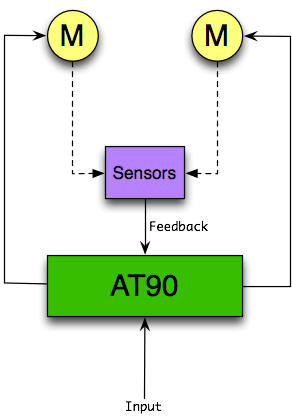
\includegraphics[width=85mm]{imageSources/pidhovercraft.png}
  \end{center}
  \caption{Hovercraft PID controller} 
  \label{pidController}
\end{figure}

Sensors are necessary to keep the hovercraft heading straight and steady and essential to the PID controller as they provide feedback information. In order to navigate the environment without running into obstacles, hovercraft will use sonars for ranging. A magnetometer to detect the heading of the hovercraft. A gyroscope to determine the angular momentum of the hovercraft, and accelerometers to detect accelerations. 

\subsubsection{Sonars}
In autonomous mode, the hovercraft can rely on the sonars in front and on either sides to determine which direction to go. For example, it will always head towards the direction as the sonar that returns the highest range. Combining such simple heuristic and magnetometer can provide precise heading for the PID controller to steer and correct the hovercraft. 

\subsubsection{Magnetometer}
The magnetometer is very crucial for both the hovercraft and the PID controller. It provides heading information of the hovercraft. Such information aid the PID controller in correcting the heading by adjusting the speed of the motors(plants) when the hovercraft is straying off course. 

\subsubsection{Gyroscopes and Accelerometers}
Collectively an unit that consists of both gyroscopes and accelerometers is called an inertia measurement unit (IMU). The gyroscope provides the rate at which the hovercraft is rotating. The angular velocity provided by the gyroscope is, in essence, the derivative term of the PID controller. Recall that the derivative term describes the rate of the change in the error. If the hovercraft is supposed to be going straight forward but it starts to yaw due to imbalance in the system, the gyroscope can provide the angular velocity of the yaw in an instantaneous time.

The accelerometers, on the other hand, ensures the hovercraft is in motion. There can be a case where the PID controller is correcting the heading by varying the speed of the motors, but the combine of the motors is not enough to propel the hovercraft forward.

\subsection{A PID Implementation in Python}
The following code sample illustrates a simple PID controller implemented in the Python programming language.  
\begin{lstlisting}[language=python]
prevError  = 0
totalError = 0

def updatePid(setPoint, processVar):  
	kP = 0.3  
	kD = 0.03  
	kI = 0.4  
	global totalError, prevError  
  
	error = setPoint - processVar  
	totalError += error  
	proportionalTerm = kP * error  
	derivativeTerm   = kD * (error - prevError)  
	integralTerm     = kI * totalError  
	prevError        = error  
  
	return proportionalTerm + derivativeTerm + integralTerm  
  
def main():  
	setPoint = 20  
	pv = 0  
    
	for i in range(0, 200):  
		pv = updatePid(setPoint, pv)  
		print 'Iteration: %d, %f' % (i, pv)

if __name__ == '__main__':  
	main()
\end{lstlisting}

The output for this program is as follows:
\begin{verbatim}
	Iteration: 0, 14.600000
	Iteration: 1, 11.342000
	Iteration: 2, 16.318340
	Iteration: 3, 16.051072
	Iteration: 4, 17.868132
	Iteration: 5, 18.113231
	Iteration: 6, 18.841568
	Iteration: 7, 19.071943
	Iteration: 8, 19.388992
	Iteration: 9, 19.535680
	Iteration: 10, 19.682512
	Iteration: 11, 19.765453
	Iteration: 12, 19.836307
	Iteration: 13, 19.880891
	Iteration: 14, 19.915947
	Iteration: 15, 19.939337
	Iteration: 16, 19.956935
	Iteration: 17, 19.969056
	Iteration: 18, 19.977962
	Iteration: 19, 19.984202
	Iteration: 20, 19.988729
	Iteration: 21, 19.991931
	Iteration: 22, 19.994238
	Iteration: 23, 19.995877
	Iteration: 24, 19.997054
	Iteration: 25, 19.997893
	Iteration: 26, 19.998495
	Iteration: 27, 19.998924
	Iteration: 28, 19.999231
	Iteration: 29, 19.999450
	Iteration: 30, 19.999607
	Iteration: 31, 19.999719
	Iteration: 32, 19.999799
	Iteration: 33, 19.999856
	Iteration: 34, 19.999897
	Iteration: 35, 19.999927
	Iteration: 36, 19.999948
	Iteration: 37, 19.999962
	Iteration: 38, 19.999973
	Iteration: 39, 19.999981
	Iteration: 40, 19.999986
	Iteration: 41, 19.999990
	Iteration: 42, 19.999993
	Iteration: 43, 19.999995
	Iteration: 44, 19.999996
	Iteration: 45, 19.999997
	Iteration: 46, 19.999998
	Iteration: 47, 19.999999
	Iteration: 48, 19.999999
	Iteration: 49, 19.999999
	Iteration: 50, 20.000000
	Iteration: 51, 20.000000
	...
	Iteration: 197, 20.000000
	Iteration: 198, 20.000000
	Iteration: 199, 20.000000
\end{verbatim}

The values, at first, oscillate for a few iterations, then they slowly converge to the set point value. Staring at the 50th iteration until the 200th iteration, end of the for loop, the output of the controller stays at the set point value. By tweaking the constant values for Kp, Kd, and Ki, one can see how the output behavior changes. 

The goal of this document is to provide a possible solution to our imbalance problems. In recent testing we have determined that uneven weight distribution is not the sole contributor to the control difficulties we are facing. It turns out that the main fan feeding air into the plenum chamber is also a contributor. At full power, this fan forces more air into the chamber, than when it's power source is partially drained. We believe that a PID controller, finely tuned to address these issues will give us the control we need to maneuver the vehicle in close quarters.

\clearpage
\section{Embedded Software for Automation}
\label{embeddedSoftwareAutomation}

\subsection{UART Implementation}
The UART is interrupt driven. The interrupt fires when you call uart\_write(uint8\_t*, int) to signify that the buffer is non empty by setting a non empty flag. There are two pointers that point at the beginning and end of the buffer, head and tail. Each character/byte is sent individually until the head == the tail and the empty flag is restored.

\lstset{language=c}
\lstset{commentstyle=\textit}
\begin{lstlisting}[frame=trbl]{}
int uart_write(uint8_t* const str, int len){
    int overflow = 0;
    int i;

    uint8_t sreg;
    sreg = SREG;

    Disable_Interrupt();
    overflow = 0;
    for(i = 0; i < len; ++i){  
        if(non_empty && head == tail) overflow = -1;

        uart_TX_buf[tail] = str[i];

        ++tail;
        tail &= UART_TX_BUF_MASK;
    }
    
    if(overflow) head = tail;     

    if(len > 0) {

        TXIntEnable();
        non_empty = 1;
    }

    SREG = sreg;
    return overflow; 
}

/**
 * Interrupt service routine for the UART transmission.
 */
ISR(USART1_UDRE_vect) {
    UDR1 = uart_TX_buf[head];
    ++head;
    head &= UART_TX_BUF_MASK;
    // Last byte was written?
    if (head == tail){
        non_empty = 0;
        TXIntDisable();
    }
}
\end{lstlisting}

The simplist way for UART to be used, is to create a character buffer and insert the desired String using sprinf. This made is very simple to monitor length and insert decimals. 

\lstset{language=c}
\lstset{commentstyle=\textit}
\begin{lstlisting}[frame=trbl]{}
int len = sprintf((char *)toPrint, "X %d, Y %d\r\n", packet->x, packet->y);
uart_write((uint8_t*)toPrint, len);
\end{lstlisting}

\subsection{DC Motor Implementation}

\subsubsection{Initialization}
The D/C motor uses Pulse Width Modulation(PWM) to determine the speed at which it turns. This PWM is sent through the enable pin of the H-bridge. There is also a direction pin which must be set to either high or low.

This pin is set as output to be able to turn the motor on and off.
\lstset{language=c}
\lstset{commentstyle=\textit}
\begin{lstlisting}[frame=trbl]{}
 DDRD |=  (1< < PORTD7);
\end{lstlisting}

This pin is the direction pin, also set to output. 

\lstset{language=c}
\lstset{commentstyle=\textit}
\begin{lstlisting}[frame=trbl]{}
 DDRC |= (1< < PORTC1);
\end{lstlisting}

Finally, this pin is the pin that outputs the PWM, also set for output. 

\lstset{language=c}
\lstset{commentstyle=\textit}
\begin{lstlisting}[frame=trbl]{}
DDRB |= (1< < PORTD7);
/** setup timer/counter 0  for fast PWM   **/ 
TCCR0A = (1 < < WGM00) | (1 < < WGM01) | (0 < < COM0A0) | (1 < < COM0A1);
TCCR0B = (0 < < WGM02) | (0 < < CS02) | (0 < < CS01) | (1 < < CS00);
\end{lstlisting}

The COM0A1..0 pins control the output of OCA0. In the motor driver, the compare output mode is set to clear OC0A when the counter matches the value in the output compare register, OCR0A, and to pull high when the counter reaches the TOP value. By setting and clearing OCA0, the pulse width that drives the motor is generated. According to the AT90USB1287 datasheet, different modes of operation will have different effect on the behavior of OC0A. The operation mode we are using is Fast PWM mode. It can be set by setting WGM02..0 to 011. The last thing that the motor initialization function does to set the clock prescaler. CS02..0 determines the prescale factor. For us, we set CS02..0 to 001 which disables the prescaling.

\begin{figure}[h]
  \begin{center}
    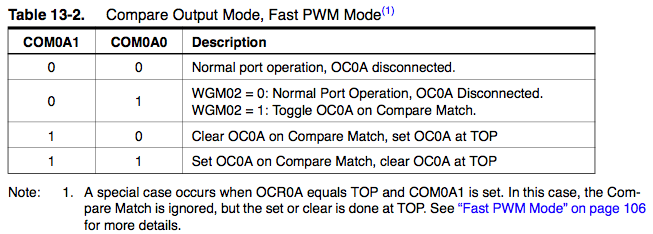
\includegraphics[width=125mm]{imageSources/pwmTable1.png}
  \end{center}
  \caption{Fast PWM Mode} 
  \label{pwmTable1}
\end{figure}

The above table outlines the 8 different types of  Waveform generation that are available. As can be seen by how we set the code, we chose to use mode7. This describes that the system uses fast PWM and that the top value is defined by OCRA.  As can be seen in the following section, we change the value of OCR0A to  change the speed of the motor.

\begin{figure}[h]
  \begin{center}
    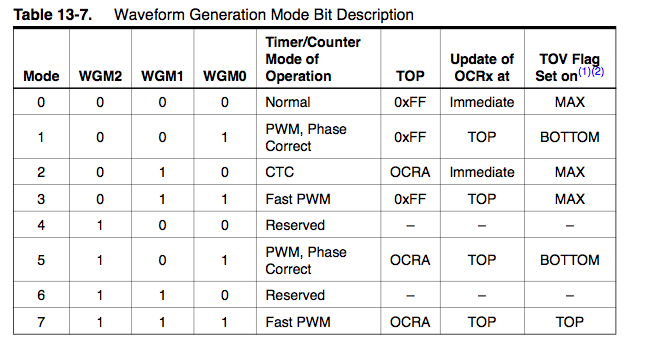
\includegraphics[width=125mm]{imageSources/waveformGenerationTable.png}
  \end{center}
  \caption{Waveform Generation Mode Bit Description} 
  \label{waveformGenerationTable}
\end{figure}

\subsubsection{Control}
To control the speed of the D/C motor, we use the function called setMotorSpeed(uint8\_t). The duty parameter sets the duty cycle period of the pulse. The larger the duty cycle is, the faster the motor will spin. 

\lstset{language=c}
\lstset{commentstyle=\textit}
\begin{lstlisting}[frame=trbl]{}
 void setMotorSpeed(uint8_t duty) {
	OCR0A = duty;
}
\end{lstlisting}

Aside from the speed of the D/C motor, we need to have control of direction of which the motor will spin. In the motor driver code, there is a function called, setMotorDirection(int), which can be used to set the direction. 

\lstset{language=c}
\lstset{commentstyle=\textit}
\begin{lstlisting}[frame=trbl]{}
void setMotorDirection(int d) {
    if (d == BACKWARD)
        PORTC |= _BV(PORTC1);
    else
        PORTC &= ~(_BV(PORTC1));
}
\end{lstlisting}

This code will either set the C1 pin High or Low. By doing this, the switches change on the H-bridge. See the explanation of H-Bridge in the design portion. 

\subsection{Joystick Implementation}
The joystick is sampled every second. The x, y, and z values of the joystick is sent via the radio from the base station to the hovercraft. On the hovercraft end, it will translate those x, y, and z values into speed/direction of the motor as well as the the degree of which the servo motor should turn. The x, y, and z values from the joystick is converted into digital signals by using the analog to digital converter (ADC) built into the AT90USB1287. Please refer to the joystick section of Hardware Overview.

\subsubsection{Analog-to-Digital Conversion}
To start a conversion from an analog signal to a digital signal, both ADEN (bit 7) and ADSC (bit 6) need to be set in the ADC Control and Status Register A (ADCSRA). As shown in the following code snippet.
\lstset{language=c}
\lstset{commentstyle=\textit}
\begin{lstlisting}[frame=trbl]{}
#define TAKE_SAMP (_BV(ADEN) | _BV(ADSC))
ADCSRA = TAKE_SAMP;
\end{lstlisting}

Since there are three inputs (x, y, and z) from the joystick,  the ADC multiplexer(ADMUX) is used to select which input value for the ADC to sample.

\lstset{language=c}
\lstset{commentstyle=\textit}
\begin{lstlisting}[frame=trbl]{}
// X value
#define SAMP0 	(_BV(REFS0) | _BV(ADLAR) | PINF1)
// Y value
#define SAMP1 	(_BV(REFS0) | _BV(ADLAR) | PINF2)
// Z value
#define SAMP2 	(_BV(REFS0) | _BV(ADLAR) | PINF4)
\end{lstlisting}

The bit ADSC is also used to determine if a conversion is in progress. It will stay high as long as there is an ongoing conversion; as soon as the conversion is completed it will become low. The following function demonstration how to use the ADSC to determine when to read the ADC results from the ADCH register. The result of the conversion can be found in the ADC Result Register (ADCL, ADCH) which is a 16-bit register. If the ADLAR bit in ADMUX register is set to high, the result is left adjusted, which means one can read the result from ADCH. If, however, the ADLAR bit is low, the result is right adjusted, so the result will be stored in ADCL.

\lstset{language=c}
\lstset{commentstyle=\textit}
\begin{lstlisting}[frame=trbl]{}
#define ADC_NOT_DONE() 	(ADCSRA & _BV(ADSC)) 
static void single_sample(unsigned char SAMPN, int input_num) {
	ADMUX = SAMPN;
	//need to sample multiple times, because A/D seems to have some
	//memory of the previous value that was read

	ADCSRA = TAKE_SAMP;
	while (ADC_NOT_DONE()){}
	ADCSRA = TAKE_SAMP;
	while (ADC_NOT_DONE()){}
	ADCSRA = TAKE_SAMP;
	while (ADC_NOT_DONE()){}

	sum[input_num] = ADCH;
}
\end{lstlisting}

\subsection{Servo Implementation}
Similar to the DC motor, the servo motor is controlled by pulse width modulation. Initializing the servo driver is very similar to the DC motor initialization function. First, a clock prescaler is chosen by setting the CS02..0 bits in TCCR1B. In the servo driver code, CS02..0 is set to 010 which sets the prescale factor to 8 or the clock is running at 1Mhz. Also we set the waveform generation mode to fast PWM mode by setting WGM13..0 to 1110. As for the output to the servo, we configure the OC1B pin to go high when the timer/counter is equal to OCR1B (= 800), and OC1B pin to go low when the timer/counter equals to ICR1 (=20000). Such configuration is done through setting COM1B1..0 pins to 10.

\lstset{language=c}
\lstset{commentstyle=\textit}
\begin{lstlisting}[frame=trbl]{}
void
servoInit(void){

	TCCR1B = (0 < < CS10)|(1 < < CS11)|(0 < < CS12)|(1 < < WGM13)|(1 < < WGM12);

	TCCR1A = (0 < < WGM10) | (1 < < WGM11) | (1 < < COM1B1) | (0 < < COM1B0);
	/*Set the IO pins for output for  OCB1*/
	DDRB = 0xFF;
	/* Set the TOP value to 2500 this should mean that the TCNT1 counter
	 should reset itself every 50 Hz at a clock of 1Mz for 8 Mhz, set to 20000(hopefully)*/
	ICR1 = 20000;
	/* Set the low timings for the three output pins for ports A in OCR1A*/
	OCR1B = 800; //corresponds to 8% duty cycle or 2ms pulse width
}
\end{lstlisting}

After initialization and configuration, the servo can be easily controlled by setting the OCR1B register.

\lstset{language=c}
\lstset{commentstyle=\textit}
\begin{lstlisting}[frame=trbl]{}
int servoDuty(int duty){
	OCR1B = duty;
	return duty;
}
\end{lstlisting}

\subsection{Sonar Implementation}
There are two stages when it comes to how the sonar operates. The first stage, the sonar sends out seven 42Khz pulses. Then, the second stage, is to the use the echoes and the PW pin on the sonar to get a pulse width representation of range. Aside from using the pulse width representation, MaxSonar can also use the TX pin to asynchronous deliver range information in RS232 format. There is another option available to acquire range data from the MaxSonar---using the ADC built into the AT90USB; the AN pin on the MaxSonar will output 0 to 2.55 volts with a factor of 10mV per inch

The sonar driver we are using uses the pulse width method. In the pulse width method, the duration of the duty cycle is used to determine the range. According the datasheet 1 inch is equal to 147uS. Since the duration is the key factor in order to determine the range, an input capture unit is used to determine the time of which the signal is pulled high as well as the time of which the signal goes low. Once the two timestamps are known, we can calculate the difference, determine the duration and range. The input capture unit is found in one of the 16-bit timers (we are using timer 3). Hence the initialization is pretty similar to other peripherals aforementioned.

\subsubsection{Initialization}
The first initialization step is to set the clock source and choose a clock prescaler. The clock prescale factor is chosen by setting CS32..0 bits in the Timer/Counter3 Control Register (TCCR3B) to 010 which translates to the system clock speed divided by 8 (=1Mhz). After the clock source is set, we choose to enable the noise canceler by setting the ICNC3 bit in TCCR3B. Enabling the noise canceler allows for more reliable range data with the cost of four system clock cycles of delay, because the canceler will take four samples, and all of those four samples have to be of equal value before the change is propagated to the edge detector which might then triggers an interrupt. In order to get notified about the incoming range information from the sonar, the input capture interrupt is used. First, we need to determine which edge on the Input Capture Pin (ICP3) will trigger an event. When an event is triggered the counter value will be stored in the Input Capture Register 3 (ICR3) and the corresponding Input Capture Flag 3 (ICF3) bit is set. The ICF3 bit may then optionally cause an interrupt to fire, only if the input capture interrupt is enabled. In the initialization code, an event is set to trigger whenever a rising edge is detected. This is done by setting the ICES3 bit in TCCR3B register to high. Next, the input capture interrupt is enabled as well as the ICF3 bit in the Timer/Counter3 Interrupt Flag Register 3 (TIFR3) is cleared (Note: ICF3 bit is cleared by writing a logic one to its bit location). The last thing the initialization code does is to let the sonar performs a calibration cycle by setting the RX pin (PINC7) high.

\lstset{language=c}
\lstset{commentstyle=\textit}
\begin{lstlisting}[frame=trbl]{}
#define SONAR_PORT      PORTC
#define SONAR_ECHO_MASK (_BV(7))                                        
void sonar_init(){
//      initialize sonar
	DDRC |= _BV(7);                       
    TCCR3B &= ~(_BV(CS32) | _BV(CS30));     
    TCCR3B |= _BV(CS31);                            
    TCCR3B |= _BV(ICNC3);                           
//      enable timer and global interrupts
    TCCR3B |= _BV(ICES3);
    TIFR3  |= _BV(ICF3);
    TIMSK3 |= _BV(ICIE3);
    PORTC |= _BV(7);
    sei();
	int i=0;
    for(i=0; i < 63; ++i) _delay_ms(40);
}
\end{lstlisting}

\subsubsection{Range Calculation}
The majority of the calculation is done through the input capture interrupt. The ISR will determine what triggers the event. If it is an rising edge that triggers the event, it will set the set the counter to 0. Then the behaviour of the input capture interrupt is changed so that the interrupt will fire on a falling edge. In order to change the input capture interrupt behaviour the ISR sets the ICES3 bit to 0. After updating the interrupt firing behaviour, the input capture flag is cleared. According to the AT90USB1287 data sheet, the ICF3 bit must be cleared every time an edge changes (Again, ICF3 is cleared by writing a logical one to the corresponding bit location). After a rising edge is detected, the timer/counter is to set to 0 and the interrupt is configured to fire when a falling edge is detected. If a falling edge occurs, the timestamp will saved to the ICR3 register. In the ISR, when the triggering event is a falling edge event, the timestamp is read from ICR3 and stored to a global variable called, time\_falling, which essentially is the duration of the duty cycle. Then the input capture interrupt is changed back to detect a rising edge.

\lstset{language=c}
\lstset{commentstyle=\textit}
\begin{lstlisting}[frame=trbl]{}
#define IS_RISING_EDGE()   (TCCR3B & _BV(ICES3))
#define IS_FALLING_EDGE()  ~(TCCR3B & _BV(ICES3))
#define SET_RISING_EDGE()  (TCCR3B |= _BV(ICES3))                          
#define SET_FALLING_EDGE() (TCCR3B &= ~(_BV(ICES3)))                       
#define CLEAR_IC_FLAG()    (TIFR3 |= _BV(ICF3))
ISR(TIMER3_CAPT_vect) {
	DISABLE_PULSE();                                        
	recieved = 1;
	if (IS_RISING_EDGE()) {
		TCNT3=0;
		SET_FALLING_EDGE();
		CLEAR_IC_FLAG();
	} else {
		time_falling = ICR3;                    
		SET_RISING_EDGE();
		CLEAR_IC_FLAG();
	}	
}
\end{lstlisting}

Finally, the actual distance can be calulated by divding the duration of the duty cycle by 147 (which is given by the MaxSonar datasheet). The result will be the distance in inches.

\lstset{language=c}
\lstset{commentstyle=\textit}
\begin{lstlisting}[frame=trbl]{}
#define US_PER_INCH 147
uint8_t read_distance() {
	return (time_falling/US_PER_INCH);      
}
\end{lstlisting}

\subsection{Radio Implementation}
The radio driver we are using are quite straight forward to use. But it is quite involved when it comes to configurating the radio. Before using the radio driver, we have to determine the addresses and the channel to be used by the base station and the hovercraft. For the base station, we have chosen the address 0xDEAD and for the hover station, the address 0xFACE is used. The radio units will be operating on channel 115.

\subsubsection{Radio Modes}
The TRW-24G radio unit we are using has three primary modes and a few sub-modes. Those primary modes as well as the pin settings for changing into a particular mode is listed below.

\begin{figure}[h]
  \begin{center}
    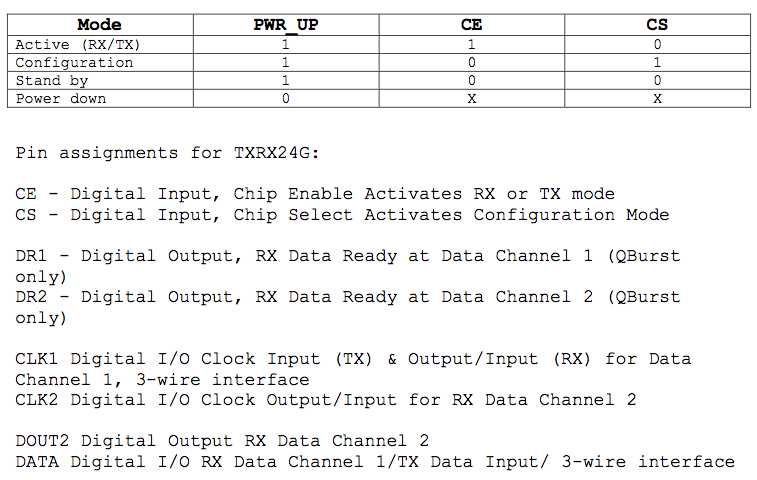
\includegraphics[width=125mm]{imageSources/radioModes.png}
  \end{center}
  \caption{Radio Modes} 
  \label{radioModes}
\end{figure}

\subsubsection{Radio Initialization and Configuration}
Before the radio can be used to transmit data, it has to be configured. The configuration involves setting the radio address, setting the operation mode (receive mode or tranmit mode), as well as other configurations which can be found in the radio's datasheet. In total, the configuration word can be up to 15 bytes long. An overview of the configuration is shown below.

\begin{figure}[h]
  \begin{center}
    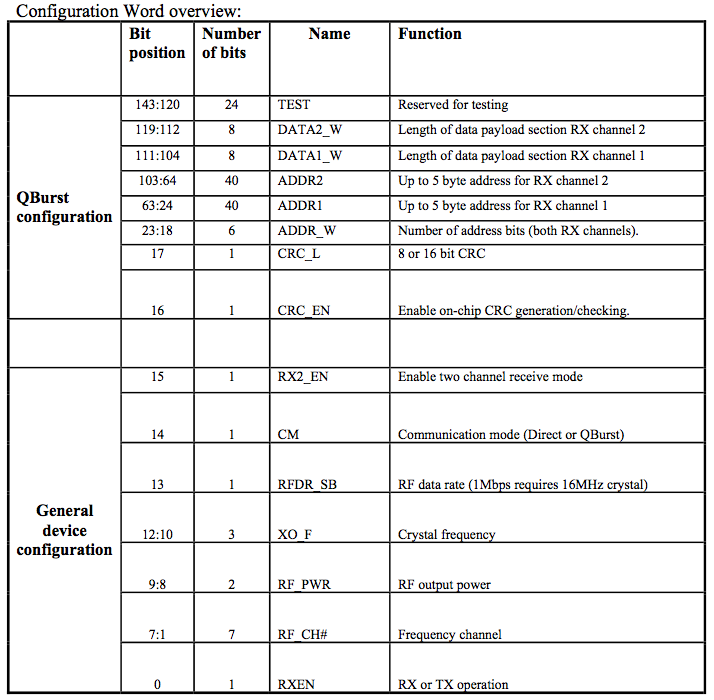
\includegraphics[width=125mm]{imageSources/radioConfigOverview.png}
  \end{center}
  \caption{Radio: Word Configuration Overview} 
  \label{radioConfigOverview}
\end{figure}

The majority of the radio initialization code is to deal with the configuration of the radio, but at the end of the radio\_init function, INT4 is enabled such whenever a packet arrives, the ISR can handle it.

\lstset{language=c}
\lstset{commentstyle=\textit}
\begin{lstlisting}[frame=trbl]{}
int radio_init(uint16_t address, uint8_t rx_enable)
{
   // ...
   // For brevity most of configuration code is cut out.
   set_rxtx_mode();

   /* Enable external interrupt on INT4 when in RX mode */
   if (rx_enable)
   {
      EIMSK |= _BV(INT4);
   }
   return 0;
}
\end{lstlisting}

\subsubsection{Sending and Receiving}
The radio driver relies on interrupt 4 (INT4) to receive packets and for sending packets, the radio must switch to transmit (if it isn't already), then the function radio\_send() can be used to send out packets. In the INT4's ISR, the packet is read one byte at a time into a buffer, then the buffer can be interpreted in any way you see fit. Since TRW24G is a half-duplex radio, the radio must be set to receive mode before it can receive any packets, and vice versa for the sending out packets.

\lstset{language=c}
\lstset{commentstyle=\textit}
\begin{lstlisting}[frame=trbl]{}
void radio_set_transmit(void)
{
   set_config_mode();
   put_byte(RADIO_CHANNEL << 1);
   set_standby_mode();

   /* Set DATA pin to output */
   DATA_DDR |= _BV(DATA_PINNUM);

   /* Disable external interrupt on INT4 */
   EIMSK &= ~(_BV(INT4));

   set_rxtx_mode();
} 


void radio_set_receive(void)
{
   int i;

   set_config_mode();
   put_byte((RADIO_CHANNEL << 1) | 0x1);
   set_standby_mode();

   /* Set DATA pin to input */
   DATA_DDR &= ~_BV(DATA_PINNUM);

   /* Enable external interrupt on INT4 */
   EIMSK |= _BV(INT4);

   set_rxtx_mode();

   for (i=0; i<250; ++i)
   {
      delay_1us(); // Tsby2rx = 202 us
   }
}
\end{lstlisting}

The radio mode is set through the configuration word mentioned in the configuration section. The key bit is the 0 bit of the first byte of configuration word. When the 0 bit is set to 1, then the radio is receive and if the 0 bit is 0 the radio will operate in transmit mode.

Due to a bug in the radio driver, the radio\_set\_receive() function must be called twice in order to switch the radio into receive mode. Fail to do so may leave the radio in an unknown and unoperable state.
\clearpage
\section{Real Time Operating System (RTOS)}
A Real Time Operating System (RTOS), is an operating system that must be able to
deal with time and event sensitive activities. The RTOS is intended
to be \textit{predictable} and \textit{determinant}\cite{RTOSMantis}. These
systems are also designed to limit the amount of overhead that is required to
context switch between tasks. This is done my making many critical decisions
prior to runtime.

\subsection{Tasks}

There are three different types of tasks in the RTOS; system tasks, periodic tasks and round robin tasks. These tasks are ordered in decreasing priority levels.

\begin{description}
    \item[System Tasks]
    System tasks are of the highest priority. If a system task is
    scheduled to run, it will preempt any other task.

    \item[Periodic Tasks]
    Periodic tasks are the next level below system tasks---middle priority.
    These tasks are scheduled to run periodically based on time (clock cycles).
    Periodic tasks are declared at the beginning of the program. A \texttt{PPP}
    array is also declared. This array allots time to each task and also
    declares an order for the periodic tasks. A periodic task is not allowed to
    take more time than has been allotted.  If this occurs, it is called a
    timing violation, and the system halts.

    \item[Round Robin Tasks]
    The final level---low priority -- consists of the round robin tasks. Round robin (RR) tasks
    are executed in the \textit{idle} time between periodic tasks.  The kernel
    maintains a FIFO queue containing all of the round robin tasks. On each clock
    cycle, if the system is not attending to either a system or periodic task then
    the next RR task is removed from the queue and is run for exactly one tick
    after which it is returned to the end of the FIFO queue. On the next cycle, if
    the higher priority tasks have not regained control, then the proceeding RR
    task is removed from the queue and executed.  
\end{description}



\subsection{Events and Timeouts}

System and round robin tasks are capable of waiting for an event, a timeout, or
either. The reason that only system and round robin tasks are allowed to wait on events is that if a periodic task waits longer than its time allowance, a timing violation will occur. \\

\noindent{\bf Events}\\
Events are initiated at the beginning of the program. Tasks that wait for an event are placed on a queue. The first item in the queue will continue when another task \textit{signals} that event. All of the elements will be released from the queue if another task \textit{broadcasts} that event. \\

\noindent{\bf Timeouts}\\
The kernel maintains a variable \textit{now} indicating how many ticks have occurred since program instantiation. When a task waits a certain amount of time, it will return normal operation after n ticks have passed.





The RTOS used for this project was created by Scott Craig and Justin Tanner \cite{RTOSSJ}. This RTOS is written in a mixture of C and assembly and is primarily written to support periodic tasks.   






\subsection{Tasks for Hovercraft 1---The leader}
In this project, hovercraft 1 assumes the role of a leader. It will navigate the
environment and make decisions to traverse the environment. Those decisions are then relayed to the trailing hovercraft, hovercraft 2. As a result, the implementation of hovercraft 1 is quite complex. This section will explain the
breakdown of the tasks in the implementation of hovercraft 1.

\begin{lstlisting}[float=th,label=lst:h1ppp,
                   caption={\texttt{PPP} array and task creation for hovercraft 1}]
const unsigned char PPP[] = {FIRE, 4, LISTEN, 1, FIRE, 4, LISTEN, 1, FIRE, 4,
LISTEN, 1, MOTOR, 5, RADIO, 8};
    Task_Create((void*)(&motor_task),0, PERIODIC, MOTOR);
    Task_Create((void*)(&fire_sonar),0, PERIODIC, FIRE);
    Task_Create((void*)(&listen_sonar),0,PERIODIC, LISTEN);
    Task_Create((void*)(&sendRadio),0,PERIODIC, RADIO);
	Task_Create((void*)(&stopSystem), 0,SYSTEM, STOP); 
\end{lstlisting}
The \texttt{PPP} array of hovercraft 1 and the task creation for the 5 tasks are shown in listing \ref{lst:h1ppp}.
There are in total four tasks, the first six items in the PPP array are the
two sonar tasks that are responsible for triggering and listening
to the three sonars. The integration of the sonar and the RTOS is based on the report by Will
Logan, Cambria Hanson and Jason Kereluk \cite{autoB}. In listing \ref{lst:h1sonarfire}, the implementation of the
\texttt{FIRE} task uses the built-in \texttt{Task\_Next()} function to trigger
the three sonars one by one. First, the task will trigger the front sonar, then
it will give up the CPU and allow the listen task (as shown in listing
\ref{lst:h1sonarlisten}) to calculate the distance. When the distances are
stored in their respective variables, the \texttt{MOTOR} task will run. Within
the \texttt{MOTOR} task, it will decide what speed the two motors should spin.
The code for the \texttt{MOTOR} is shown in listing \ref{lst:h1motor}. After
this, the radio task reports to both the base station and the follower
hovercraft. Listing \ref{lst:h1radio} illustrates this code. In this radio task, a test is set up to see if
three send tasks are sent before an ack is received. If this happens then the
program exits.

\begin{lstlisting}[float=thp,label=lst:h1sonarfire,
                   caption={\texttt{FIRE} Task}]
void fire_sonar(void) {
	for(;;) {
		trigger_sonar(FRONT);
		Task_Next();
		trigger_sonar(RIGHT);
		Task_Next();
		trigger_sonar(LEFT);
		Task_Next();
	}
}
\end{lstlisting}

\begin{lstlisting}[label=lst:h1sonarlisten,float=tbh,
                   caption={\texttt{LISTEN} Task}]
void listen_sonar(void) {
	for(;;)	{
	    s_forward= read_distance();
	    Task_Next();
	    s_right = read_distance();
	    Task_Next();
	    s_left = read_distance();
	    Task_Next();
	}
}
\end{lstlisting}

\begin{lstlisting}[label=lst:h1motor,float=th,
                   caption={\texttt{MOTOR} Task}]
void motor_task(void) {
	for(;;) {
    	if(s_front < MIN_DISTANCE &&  s_left >MAX_DISTANCE) {
            r_dir= FORWARD;
            r_duty = 255;
            l_dir = BACKWARD;
            l_duty = 255;
   		} else if (s_front < MIN_DISTANCE && s_right>MAX_DISTANCE) {
            r_dir = BACKWARD;
            r_duty = 255;
            l_dir= FORWARD;
            l_duty = 255;					
    	} else if (s_left < MIN_DISTANCE && s_right > MAX_DISTNACE) {
            l_dir = FORWARD;
            l_duty = 255;
            r_duty = 0;
   	 	} else if (s_right<MIN_DISTANCE && s_left > MAX_DISTANCE) {
            r_dir = BACKWARD;
            r_duty = 255;
            l_duty = 0;
    	} else {
            Signal_Event(stop);
    	}
        setMotorDirection(&rightMotor,r_dir;
        setMotorDuty(&rightMotor, r_duty);
        setMotorDirection(&leftMotor,l_dir);
        setMotorDuty(&leftMotor, l_duty);
	}
}
\end{lstlisting}

\begin{lstlisting}[label=lst:h1radio, float=th, caption={\texttt{RADIO} Task}]

void
sendRadio(void){
    for(;;){
        sendMovements(r_duty,l_duty,r_dir,r_duty);
        reportToBase(r_speed,l_speed, s_forward, s_right, s_left);
        send ++;
        if(send == 3)
            Event_Signal(stop);
        
        Task_Next();
    }
}



\end{lstlisting}

The Gantt chart in figure \ref{gantt} represents the timing for the periodic
tasks for hovercraft 1.

%\begin{minipage}{6.5in}
        \begin{center}
        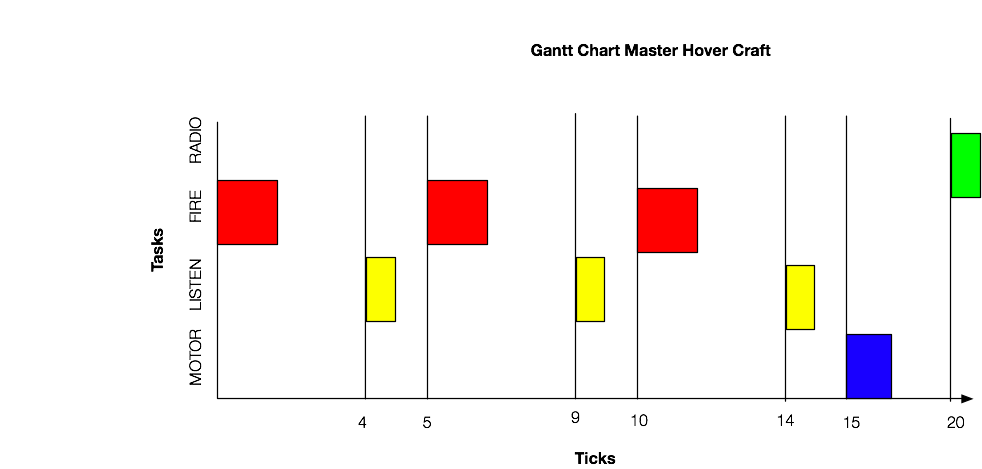
\includegraphics[width = 5.5in]{imageSources/Gantt.png}
        \captionof{figure}{Gantt chart for the master hovercraft}
        \label{gantt}
        \end{center}
%\end{minipage}

This hovercraft also has one system task. This task is responsible for
stopping the system if an error occurs and can be seen in listing \ref{lst:stop}. It attempts to stop the following
hovercraft before exiting. This system task waits for the \textit{stop} event
to be signaled.

\begin{lstlisting}[label=lst:stop, float=th, caption={\texttt{STOP} Task}]
void
stopSystem(void){
	Event_Wait(stop);
	sendMovements(0,0,FORWARD,FORWARD);
	exit(0);
}

\end{lstlisting}



\subsection{Tasks for Hovercraft 2 --- The Follower}

The second hovercraft has no periodic tasks. Most of the actions involved with
this hovercraft occur after events. As shown in in listing \ref{lst:h2setup}
there are three round robin tasks and a system task. The system task is very
similar to the system task in hovercraft 1. 


The motor and ack tasks from listing \ref{lst:h2motor} both wait on the same
event. This event occurs when a radio packet is received. This event is
broadcasted in the interrupt service routine (in listing \ref{isr} that is fired upon the detection
of an incoming packet.

The final task that belongs to this hovercraft is the pong task. This task is
part of the initial handshake. As noted in listing \ref{pong} this task does
not have a for loop, and only runs through once.

\begin{lstlisting}[label=lst:h2setup, float=th, caption={The Setup
calls for Hovercraft 2}]


        ack = Event_Init();
	pong = Event_Init();
	stop = Event_Init();

    
	Task_Create((void*)(&ack_task),0, RR, ACK);
        Task_Create((void*)(&up_motors),0, RR, MOTORS);
	Task_Creat((void*)(&pong_task),0,RR,PONG);
	Task_Create((void*)(&stopSystem), 0,SYSTEM, STOP);

 \end{lstlisting}



\begin{lstlisting}[label=lst:h2motor, float=th, caption={\texttt{MOTOR} Task}]

void
up_motors(void){

	for(;;){
		Event_Wait(ack);
                setMotorDuty(&rightMotor, rightMotorSpeed);	
                setMotorDuty(&leftMotor, leftMotorSpeed);
		setMotorDirection(&rightMotor, rightDirection);
		setMotorDirection(&leftMotor, leftDirection);
	}		
}	


void
ack_task(void){
	for(;;){
		Event_Wait(ack);
		sendACK;
	}
}

 \end{lstlisting}

\begin{lstlisting}[label=pong, float=th, caption={ISR that broadcasts Events}]
void
pong_task(void){


	Event_Wait(pong);
	sendPong();

}


 \end{lstlisting}



\begin{lstlisting}[label=isr, float=th, caption={ISR that broadcasts Events}]

ISR (INT4_vect)
{
    int i;
    
    PORTD ^= _BV(PORTD5);
    
    for (i = 0; i < PAYLOAD_BYTES; i++)
    {
        radio_buffer[i] = radio_get_byte();
    }
    
    // Figure out what type of packet this is.
    genericPacket_t *incomingPacket = (genericPacket_t *)radio_buffer;
    movePacket_t *theMovePacket;
    switch(incomingPacket->type) {
        case PING:
            pingReceived = true;
	    Signal_Event(pong);
            break;
        case MOVE:
            theMovePacket = (movePacket_t *) radio_buffer;
            rightMotorSpeed = theMovePacket->rightMotor;
            leftMotorSpeed  = theMovePacket->leftMotor;
	    rightDirection= theMovePacket-> rightDirection;
            leftDirection = theMovePacket -> leftDirection;
	    Event_Broadcast(ack);
            needSendAck = true;
            break;
        default:
            // ignore
            break;
    } 
\end{lstlisting}


\subsection{Tasks for the Base Station}

The final component to this project was a simple base station that would
report what was going on `out in the field'. This base station has one task
that is executed based on an event. This event is fired when a packet is
detected. 

The ISR is very similar to the isr in hovercraft 2 from listing \ref{isr}. It
uses event signal: \textit{Event\_Signal(radio\_event};

Listing \ref{print} shows the \textit{uart\_task} and
the \textit{printInfo(infoPacket\_t)} working together to display the
information to the screen.


\begin{lstlisting}[label=print, float=th, caption={ISR that broadcasts Events}]

void 
printInfo(infoPacket_t theInfo) 
{
    amount = sprintf(toPrint, SONAR_INFO_STRING, theInfo.frontSonar, theInfo.rightSonar,
                     theInfo.leftSonar);
    uart_write((uint8_t *)toPrint, amount);
    amount = sprintf(toPrint, MOTOR_INFO_STRING, theInfo.rightMotor, theInfo.leftMotor);
    uart_write((uint8_t *)toPrint, amount);
}


uart_task(void)
{
     for(;;)
    {
        Event_Wait(radio_event);
      	printInfo(*info);
        Task_Next();
    }
}

\end{lstlisting}

\clearpage
\section{Physical Parameters: Methodologies and Measurements}
To help gain a better understanding of the physical system, various aspects of the hovercrafts' control and motion were qualitatively and quantitatively measured and analyzed. These measurements were employed as part of the process of supplying the vehicles with autonomous intelligence. This section of the report provides details about the following parameters: maximum speed, stopping distance, PWM cycles vs actual speed and payload vs actual speed.

\subsection{Distance}
A first step in many subsequent calculations was the determination of the distance between the hovercrafts and an oncoming object. It was decided that a sonar could be used to calculate this distance. The sonar was calibrated to report the distance between itself and an object in inches.

\subsection{Speed}
To calculate the speed of the craft, sonar readings were sampled at a set interval.  The change in the values of theses readings (with respect to time) produced a reliable source means for determining the speed of the vehicles.  The most challenging aspect of this approach was accurately sampling the sonar readings at set intervals.  The procedure for sampling the sonar at set intervals in an accurate manner is as follows:

The clock speed is at 8 MHz.  Timer 2, which is an 8 bit timer, was used. The prescaler was set to a factor of 1024, resulting in a frequency reduction to 8 000 000/1024 = 7812.5Hz. A counter increased at this frequency, and thus  overflowed every 256 ticks. By setting the TOIE2 bit in the TIMSK2 register, an interrupt was enabled on each overflow. This resulted in the register overflowing 30 times per second (7812.5 / 256). In the overflow register, a counter existed that increased each time the interrupt was fired, thus maintaining a count of the cumulative overflows.  Further, a variable was maintained to represent the desired amount of time between sonar firings. This variable was set at 2, so that the sonar would fire every 2 seconds. In the overflow interrupt, an if statement checked to see if the counter had overflowed enough times for 2 seconds to pass. If this conditional returned true, the counter was reset to zero and the sonar triggered. This if statement also contained the code to calculate the current speed. An array of size two was also created that maintains the current sonar reading and the previous sonar reading. The difference was calculated between these readings and divided by two. The speed was calculated using decimal numbers. This reduced the accuracy, but saved on space from using the floating point numbers. The output was finally sent to UART.

While testing the sonar, it was noticed that significant of noise was generated when the sonar read the value of new objects. This had a significant impact on the quality of the final speed measurement generated. To account for this, we created a static array of 5 integers which holds the values of the 5 most recent speed calculations. The final speed, used by the vehicle's components, is the average of these 5 speed calculations. We found that this modification greatly improved the accuracy in the trend of speed calculations output to uart. We believe that we may be able to do even better. By eliminating values that seem to be complete noise, the average speed calculations will also be more accurate because they don't include such outliers. We hope to have this additional logic incorporated into milestone 3.

\lstset{language=c}
%\lstset{commentstyle=\textit}
\begin{lstlisting}[frame=trbl]{}
#define OVERFLOW_LIMIT 30
#define TIME_BETWEEN_SONAR 2

volatile int overflowCounter  = 0;
volatile uint8_t timeInterval = 0;
volatile uint8_t distances[2] = {0, 0};
volatile bool isSecondReading = false;

volatile char uartBuf[255];
volatile int  uartLen = 0;

void 
speedCalcInit()
{
    // Set TIMER 2 to CTC mode.
    TCCR2A &= ~(1 < < WGM20);
    TCCR2A |=(1 < < WGM21);
    TCCR2B &= ~(1< < WGM22);

    // Set clock prescaler to 1024
    TCCR2B |= (1 < < CS22) | (1 < < CS21) | (1 < < CS20);

    // Set OC2A on compare match
    TCCR2A |= (1 < < COM2A1) | (1 < < COM2A0);

    // Enable interrupt on compare match
    TIMSK2 |= (1 < < OCIE2A);

    // Enable overflow interrupt
    TIMSK2 |= (1 < < TOIE2);

    // Set OCR2A to the highest possible value.
    OCR2A = 0xFF;
}

/**
 * Compare match interrupt service routine.
 */
ISR(TIMER2_COMPA_vect)
{

}

/**
 * Timer 2 overflow interrupt service routine.
 */
ISR(TIMER2_OVF_vect)
{
    if (++overflowCounter >= OVERFLOW_LIMIT) {
        ++timeInterval;
    }

    if (timeInterval >= TIME_BETWEEN_SONAR) {
        trigger_sonar();
        timeInterval = 0;
        overflowCounter = 0;

        if (!isSecondReading) {
            distances[0] = read_distance();
            isSecondReading = true;
        } else {
            distances[1] = read_distance();

            uartLen = sprintf((char *)uartBuf, "%d\r\n", distances[0]);
            uart_write((uint8_t *)uartBuf, uartLen);
            uartLen = sprintf((char *)uartBuf, "%d\r\n", distances[1]);
            uart_write((uint8_t *)uartBuf, uartLen);

            // calcluate velocity
            int velocity = (distances[1] - distances[0])/TIME_BETWEEN_SONAR;
            uartLen = sprintf((char *)uartBuf, "vel: %d\r\n", velocity);
            uart_write((uint8_t *)uartBuf, uartLen);

            distances[0] = distances[1];
        }
    }
}
\end{lstlisting}

\subsection{Turning Radius}
The turning of our craft is very small, almost in place. To get this effect, we have two motors that are on either side of the centre. When turning at full speed, one motor will me moving forwards, while the other is spinning backwards. Table \ref{turningRadius} shows the speeds and corresponding PWMs. 

\begin{table}
\caption{Hovercraft Turning Radius}
\begin{center}
\begin{tabular}{ c c }
  Speed (inch/sec) & PWM \\
  \hline
  5 & 255 \\
  3 & 245 \\
\end{tabular}
\end{center}
\label{turningRadius}
\end{table}

Once we were accurately able to calculate the speed of the craft it was simple to calculate the stopping distance. We set up a test area in the a hallway with a tape measurer along the wall. We had two different stopping tests. In the first, we would drive the robot down the hall. Once the robot steadily reached the testing speed, we would allow the joystick to snap back into the center 'resting' position and measure the distance the robot traveled.

\subsubsection{`Resting' Stop}
\begin{table}
\caption{Stopping Distances (to rest)}
\begin{center}
\begin{tabular}{ c c }
  Speed (inch/sec) & Stopping Distance (meters) \\
  \hline
  5 & 3 \\
  3 & 2.5 \\
\end{tabular}
\end{center}
\label{restingTable}
\end{table}

The other way that the robot could stop, was by reversing both motors. We would have the same initial set up with a tape measurer in the hall way, but once the craft reached the `testing' speed, we would then pull the joystick into maximum reverse position. For this calculation we were also required to record the time it took the craft to stop. The reason we needed to do this, was so that when we are driving the robot autonomously, we are able to calculate the duration that the motors must run in reverse to come to a complete stand still with out traveling backwards.

\subsubsection{`Reverse' Stop}
\begin{table}
\caption{Stopping Distances (from Reverse)}
\begin{center}
\begin{tabular}{ c c }
  Speed (inch/sec) & Stopping Distance (meters) \\
  \hline
  5 & 1.3 \\
  3 & 0.90 \\
\end{tabular}
\end{center}
\label{reverseTable}
\end{table}

\subsection{Payload}
All of the above measurements are recorded with only the required components placed on the hovercraft, as well as the additional components required to eliminate rotational spin. The following table, describes how the speed of the craft changes with the amount of excess weight is added to the craft. All of the additional weight was distributed evenly around the chassis to minimize the rotational spin. The table also describes how the speed changes when the motors are receiving full (255) PWM.
\begin{table}
\caption{Hovercraft Supported Weight}
\begin{center}
\begin{tabular}{ c c }
  Additional Weight (grams) & Speed (meters/sec) \\
  \hline
  100 & 4 \\
  200 & 3 \\
  300 & 1 \\
  400 & stopped \\
\end{tabular}
\end{center}
\label{weightTable}
\end{table}

\clearpage
\section{Observations and Evaluations}
This section describes the outcomes of the various tests and mini-experiments that were performed as the project advances, as well as the pertinent observations made throughout.  
\clearpage
\section{Conclusion}
This project, the construction of two autonomous and coordinated hovercrafts, has served as a learning experience for many problem domains including embedded software, electrical engineering, control theory, and more.  This team's primary interests were those revolving around software problems - concerns such as inter-hovercraft communication, onboard software debugging, control synchronization, code efficiency and autonomous intelligence (for example the implementation of a PID controller).  Unfortunately, the team's tendencies and strengths in the software domain, and lack of knowledge in the hardware domain, was likely a main factor in the less-than-perfect project implementation.  

Arguably, the largest problem that impeded the progress of the project was the unwanted movement found when testing each of the hovercraft prototypes.  Factors such as rotational torque, uneven airflow from the base and skirt, nonuniform distribution of weight across the body, and unbalanced thrust from each of the propellers all contributed to unwanted movement to a hovercraft that should have been stationary.  Without this most basic level of control over the physical system, implementing a truly effective PID controller and communication scheme among master and slave hovercrafts was next to impossible.  Another problem that plagued the entire endeavor was a general lack of understanding of electronics and electrical engineering principles.  Questionable wiring and soldering, as well as unclear usage and application of several common electrical components (H-bridges, resistors, measurement equipment, etc) made many processes more painful than they should have.  Inexperience with these components and principles lead to hours of confusion, an example is when the team believed they had made a wiring mistake, or were given a faulty H-bridge, when the problem was simply that a heat-sink had to be attached, as the H-bridge was overheating. That said, the project did advance satisfactorily in many other areas.  

Communications were one of the most interesting aspects of the project.  Hovercraft-to-base communications was straightforward and was implemented in milestone 1.  Hovercraft-to-hovercraft communications were somewhat more difficult.  Successful communication in this environment required a higher degree of fault-tolerance and automation. Once the user initiates both vehicles, he or she no longer has any further control of the physical system.  The approach taken, a state diagram and protocol whereby the leading vehicle acted as the master while the following vehicle acted as a passive slave, seemed to be the most plausible and manageable solution.  In fact, 3-way communication needed to occur.  The hovercraft-to-hovercraft traffic was needed to synchronize movement among the vehicles, while master hovercraft-to-base was also required to provide monitoring diagnostic information.  While this scheme at first appears complicated, designing a well thought out state diagram and carefully implementing it resulted in satisfactory behavior.  

Another area of interest was code efficiency and correctness.  Very soon into the project, it was discovered that traditional debugging techniques simply aren't adequate for an embedded system.  An approach as elementary as inserting printf calls throughout the code was unacceptable as that function call takes too much time to execute.  Instead of a full printf call, a much simpler function was used to print a small number of characters to the microcontroller's UART I/O connection.  This form of debugging was acceptable but there were some unnecessary complexities involved including the UART support code, radio communication code, and various interrupt handlers.  An alternative that was superior for many debugging tasks was the JTAG onboard debugging option.  A JTAG unit was connected directly to the JTAG I/O connection on the Atmel microcontroller, allowing the CPU's registers to be examined directly.  This particular embedded environment is also a real-time system.  As such, the most complicated dimension of the code, by far, is meeting the stringent timing demands of the system.  The most productive way to combat this problem seemed to be incorporating a realtime operating system to help automative much of the timing logic of tasks.  The RTOS used was the in-house RTOS developed by previous students in the course.  

The following are recommendations for future students who plan on undertaking a similar project.  First, be sure to acquire a solid understanding of general electronics, wiring and measurement techniques, and schematic diagrams.  Developing the software for a system such as this is but a small fraction of the overall process required.  In fact, it may be wise to ensure that at least one team member has a significant background in electrical engineering concepts. Next, take the proper time to understand the programming environment.  Programming at such a low level is different for many reasons, a few being severely reduced hardware resources, an alternate standard C library and assembly instruction set, significant interaction at the hardware interface level, and developing an alternate way to debug and test code.  Finally, be sure to take a pragmatic approach to constructing the physical system.  Devise miniature experiments to test theories about how the system will behave.  Choose functionality over aesthetics always. Thoroughly test each component independently. Choose simplicity over complexity.  Solve as many problems as possible at the hardware level instead of delegating it to software.  For example, PID controllers are difficult enough to get right with a well behaved physical system.  Tuning a PID controller to a sporadic and unpredictable physical system is next to impossible. Document everything.  Following these recommendations should help to streamline the construction process and will serve to help one get the most of a course as diverse and challenging as this one. 
\clearpage
%ACKNOWLEDGMENTS are optional
%\section{Acknowledgments}

\bibliographystyle{abbrv}
\bibliography{bibliography}  % sigproc.bib is the name of the Bibliography in this case


\end{document}
